\documentclass[twoside,a4paper]{book}
\usepackage{graphicx}
\usepackage{hyperref}
\usepackage{amsmath}
\usepackage{amssymb}
\usepackage{textcomp}
\usepackage[utf8]{inputenc}
\usepackage[polish]{babel}
\usepackage[T1]{fontenc}
\usepackage{standalone}
\usepackage{array}
% pakiet stosowany do url'i w bibliografii, zamienia odnośniki na ładnie sformatowane
\usepackage{url}





% pakiety służące do numerowania i tworzenia algorytmów
\usepackage{algorithmic}
\usepackage{algorithm}
% redefinicja etykiety nagłówkowej listy algorytmów, domyślna jest po angielsku
\renewcommand{\listalgorithmname}{Spis algorytmów}

\usepackage[section]{placeins}
\usepackage{pdfpages}

% pakiet do wyliczania skali, przydatny przy dużych obrazkach
\usepackage{pgf}
% pakiet służący do automatycznego sortowania odnośników do bibliografii
\usepackage[sort]{natbib}

% tworzenie listingów
\usepackage{listings}
% tworzenie figur wewnątrz figur
\usepackage{subfig}
% do automatycznego skracania nazw rozdziałów i podrozdziałów używanych w nagłówkach strony by mieściły się w jednej linii
\usepackage[fit]{truncate}
% fancyhdr - ładne nagłówki, definicja wyglądu nagłówka, numery stron będą umieszczane w nagłówku po odpowiedniej stronie
\usepackage{fancyhdr}
\pagestyle{fancy}
\renewcommand{\chaptermark}[1]{\markboth{#1}{}}
\renewcommand{\sectionmark}[1]{\markright{\thesection\ #1}}



\fancyhf{}
\fancyhead[LE,RO]{\bfseries\thepage}
% tutaj ograniczamy szerokość pola w nagłówku zawierającego nazwę rozdziału/podrozdziału do 95% szerokości strony
% redefinicja sposobu prezentacji nazw domyślnie wypisywanych wielkimi literami (np. domyślnie w nagłówku Spis treści będzie miał postać SPIS TREŚCI)
% Uwaga! to może popsuć wielkie litery w ogóle! Jak coś nie działa należy usunąć \nouppercase{} z poniższych definicji
\fancyhead[LO]{\nouppercase{\bfseries{\truncate{.95\headwidth}{\rightmark}}}}
\fancyhead[RE]{\nouppercase{\bfseries{\truncate{.95\headwidth}{\leftmark}}}}
\renewcommand{\headrulewidth}{0.5pt}
\renewcommand{\footrulewidth}{0pt}

% definicja typu prostego wymagana przez pierwsze strony rozdziałów itp.
% powyższe reguły niestety tych stron nie dotyczą, gdyż Latex automatycznie przełącza je pomiędzy fancy a plain
% w tym wypadku eliminujemy nagłówki i stopki na stronach początkowych
\fancypagestyle{plain}{%
 \fancyhead{}
 \fancyfoot{}
 \renewcommand{\headrulewidth}{0pt}
 \renewcommand{\footrulewidth}{0pt}
}

\parskip 0.05in


% makro umożliwiające otaczanie symboli okręgami
\usepackage{tikz}
% brak justowania tekstu (bazą okręgu będzie linia tekstu)
\newcommand*\mycirc[1]{
  \begin{tikzpicture}
    \node[draw,circle,inner sep=1pt] {#1};
  \end{tikzpicture}}

% pionowe justowanie tekstu, środek okręgu pokrywa się ze środkiem tekstu
\newcommand*\mycircalign[1]{%
  \begin{tikzpicture}[baseline=(C.base)]
    \node[draw,circle,inner sep=1pt](C) {#1};
  \end{tikzpicture}}

% zmiana nazwy twierdzeń i lematów
\newtheorem{theorem}{Twierdzenie}[section]
\newtheorem{lemma}[theorem]{Lemat}

% tworzenie definicji dowodu
\newenvironment{proof}[1][Dowód]{\begin{trivlist}
\item[\hskip \labelsep {\bfseries #1}]}{\end{trivlist}}
% \newenvironment{definition}[1][Definicja]{\begin{trivlist}
% \item[\hskip \labelsep {\bfseries #1}]}{\end{trivlist}}
% \newenvironment{example}[1][Przykład]{\begin{trivlist}
% \item[\hskip \labelsep {\bfseries #1}]}{\end{trivlist}}
% \newenvironment{remark}[1][Uwaga]{\begin{trivlist}
% \item[\hskip \labelsep {\bfseries #1}]}{\end{trivlist}}

% definicja czarnego prostokąta zwyczajowo dodawanego na koniec dowodu
\newcommand{\qed}{\nobreak \ifvmode \relax \else
      \ifdim\lastskip<1.5em \hskip-\lastskip
      \hskip1.5em plus0em minus0.5em \fi \nobreak
      \vrule height0.75em width0.5em depth0.25em\fi}

% poniższymi instrukcjami można sterować co ma być numerowane a co nie i co ma być wyświetlane w spisie treści
% \setcounter{secnumdepth}{3}
% \setcounter{tocdepth}{5}

% definicja czcionki mniejszej niż tiny (domyślnie takiej małej nie ma)
\usepackage{lmodern}
\makeatletter
  \newcommand\tinyv{\@setfontsize\tinyv{4pt}{6}}
\makeatother

% definicja jeszcze mniejszej czcionki
\usepackage{lmodern}
\makeatletter
  \newcommand\tinyvv{\@setfontsize\tinyvv{3.5pt}{6}}
\makeatother

% pakiet do obsługi wielostronicowych tabel
\usepackage{longtable}
\setlength{\LTcapwidth}{\textwidth}

\usepackage[section] {placeins}

\usepackage{multirow}

\usepackage{slantsc}
\usepackage[labelsep= space]{caption}
\usepackage[font=small,labelfont=bf]{caption}
\usepackage[justification=centering]{caption}
\addto\captionspolish{\renewcommand{\figurename}{Rys.}}
\addto\captionspolish{\renewcommand{\tablename}{Tab.}}
\addto\captionspolish{\renewcommand*{\appendixpagename}{Dodatki}}
\addto\captionspolish{\renewcommand*{\appendixtocname}{Dodatki}}
\addto\captionspolish{\renewcommand*{\appendixname}{Dodatek}}


\usepackage{helvet}
%\renewcommand{\familydefault}{\sfdefault}


\usepackage[toc,page]{appendix}

\begin{document}
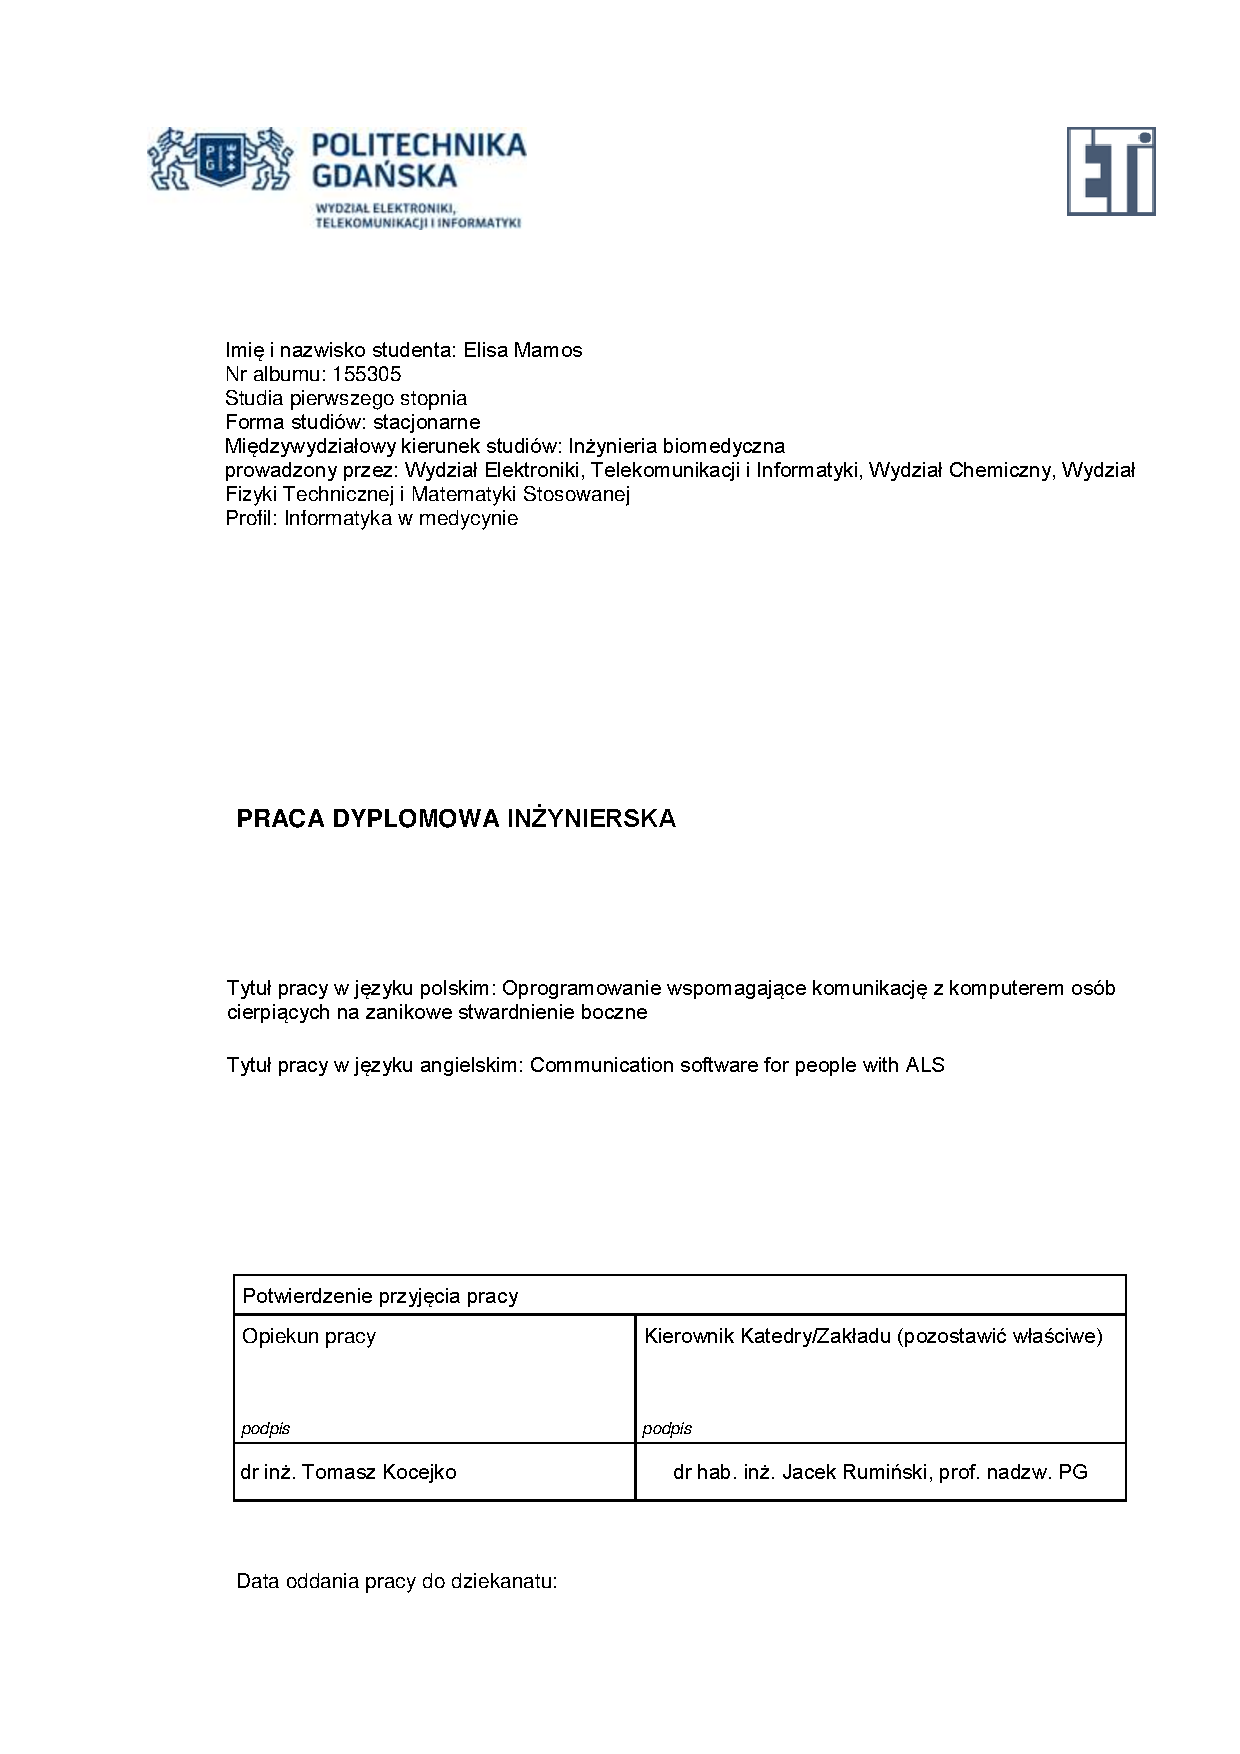
\includepdf[pages={1}]{titlePage.pdf}
\newpage
\thispagestyle{empty}
\mbox{}
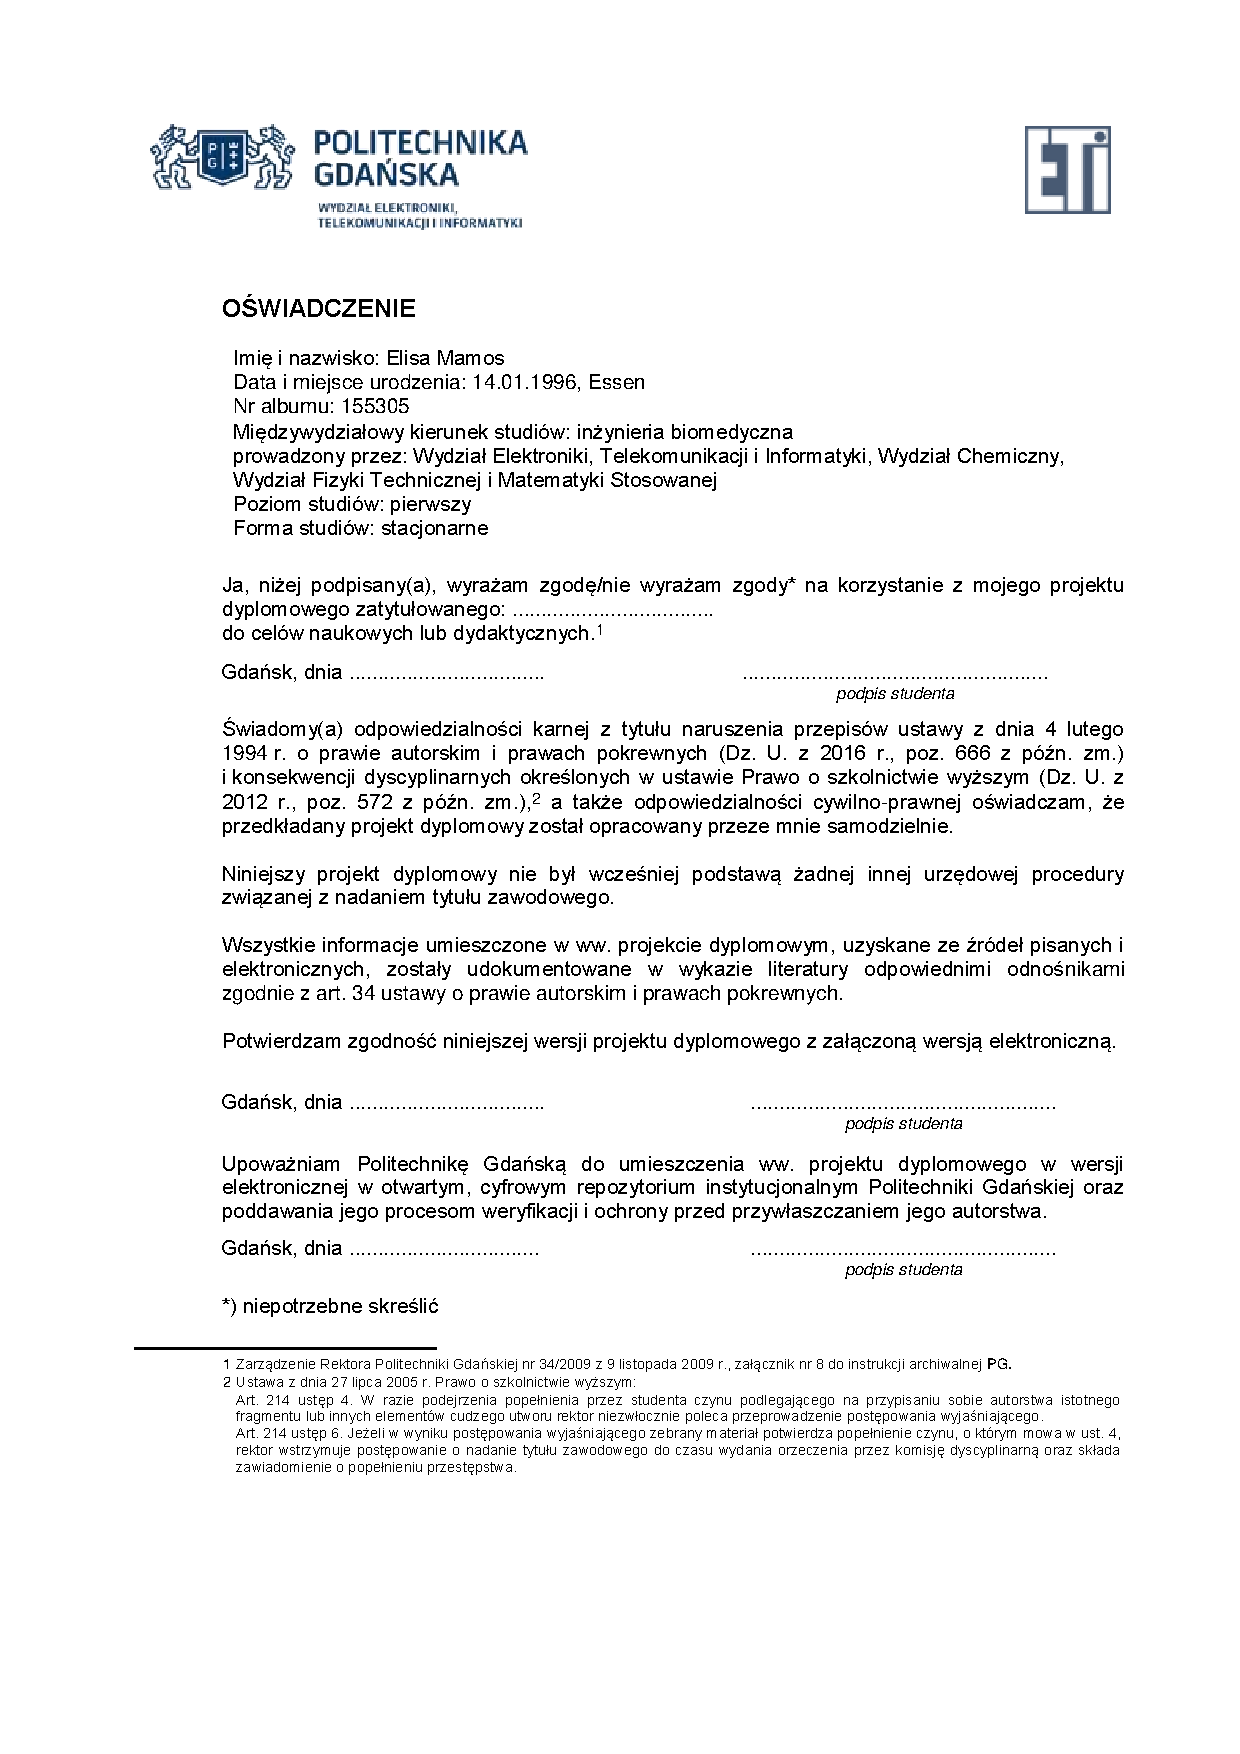
\includepdf[pages={1}]{oswiadczenie.pdf}
\newpage
\thispagestyle{empty}
\mbox{}
{\renewcommand{\addtocontents}[2]{}
\chapter*{Streszczenie}}
\tableofcontents
\documentclass[twoside,a4paper]{book}
\usepackage{graphicx}
\usepackage{hyperref}
\usepackage{amsmath}
\usepackage{amssymb}
\usepackage{textcomp}
\usepackage[utf8]{inputenc}
\usepackage[polish]{babel}
\usepackage[T1]{fontenc}
\usepackage{standalone}
\usepackage{array}
% pakiet stosowany do url'i w bibliografii, zamienia odnośniki na ładnie sformatowane
\usepackage{url}
% pakiety służące do numerowania i tworzenia algorytmów
\usepackage{algorithmic}
\usepackage{algorithm}
% redefinicja etykiety nagłówkowej listy algorytmów, domyślna jest po angielsku
\renewcommand{\listalgorithmname}{Spis algorytmów}

\usepackage[section]{placeins}
\usepackage{pdfpages}

% pakiet do wyliczania skali, przydatny przy dużych obrazkach
\usepackage{pgf}
% pakiet służący do automatycznego sortowania odnośników do bibliografii
\usepackage[sort]{natbib}
% tworzenie listingów
\usepackage{listings}
% tworzenie figur wewnątrz figur
\usepackage{subfig}
% do automatycznego skracania nazw rozdziałów i podrozdziałów używanych w nagłówkach strony by mieściły się w jednej linii
\usepackage[fit]{truncate}
% fancyhdr - ładne nagłówki, definicja wyglądu nagłówka, numery stron będą umieszczane w nagłówku po odpowiedniej stronie
\usepackage{fancyhdr}
\pagestyle{fancy}
\renewcommand{\chaptermark}[1]{\markboth{#1}{}}
\renewcommand{\sectionmark}[1]{\markright{\thesection\ #1}}



\fancyhf{}
\fancyhead[LE,RO]{\bfseries\thepage}
% tutaj ograniczamy szerokość pola w nagłówku zawierającego nazwę rozdziału/podrozdziału do 95% szerokości strony
% redefinicja sposobu prezentacji nazw domyślnie wypisywanych wielkimi literami (np. domyślnie w nagłówku Spis treści będzie miał postać SPIS TREŚCI)
% Uwaga! to może popsuć wielkie litery w ogóle! Jak coś nie działa należy usunąć \nouppercase{} z poniższych definicji
\fancyhead[LO]{\nouppercase{\bfseries{\truncate{.95\headwidth}{\rightmark}}}}
\fancyhead[RE]{\nouppercase{\bfseries{\truncate{.95\headwidth}{\leftmark}}}}
\renewcommand{\headrulewidth}{0.5pt}
\renewcommand{\footrulewidth}{0pt}

% definicja typu prostego wymagana przez pierwsze strony rozdziałów itp.
% powyższe reguły niestety tych stron nie dotyczą, gdyż Latex automatycznie przełącza je pomiędzy fancy a plain
% w tym wypadku eliminujemy nagłówki i stopki na stronach początkowych
\fancypagestyle{plain}{%
 \fancyhead{}
 \fancyfoot{}
 \renewcommand{\headrulewidth}{0pt}
 \renewcommand{\footrulewidth}{0pt}
}

\parskip 0.05in


% makro umożliwiające otaczanie symboli okręgami
\usepackage{tikz}
% brak justowania tekstu (bazą okręgu będzie linia tekstu)
\newcommand*\mycirc[1]{%
  \begin{tikzpicture}
    \node[draw,circle,inner sep=1pt] {#1};
  \end{tikzpicture}}

% pionowe justowanie tekstu, środek okręgu pokrywa się ze środkiem tekstu
\newcommand*\mycircalign[1]{%
  \begin{tikzpicture}[baseline=(C.base)]
    \node[draw,circle,inner sep=1pt](C) {#1};
  \end{tikzpicture}}

% zmiana nazwy twierdzeń i lematów
\newtheorem{theorem}{Twierdzenie}[section]
\newtheorem{lemma}[theorem]{Lemat}

% tworzenie definicji dowodu
\newenvironment{proof}[1][Dowód]{\begin{trivlist}
\item[\hskip \labelsep {\bfseries #1}]}{\end{trivlist}}
% \newenvironment{definition}[1][Definicja]{\begin{trivlist}
% \item[\hskip \labelsep {\bfseries #1}]}{\end{trivlist}}
% \newenvironment{example}[1][Przykład]{\begin{trivlist}
% \item[\hskip \labelsep {\bfseries #1}]}{\end{trivlist}}
% \newenvironment{remark}[1][Uwaga]{\begin{trivlist}
% \item[\hskip \labelsep {\bfseries #1}]}{\end{trivlist}}

% definicja czarnego prostokąta zwyczajowo dodawanego na koniec dowodu
\newcommand{\qed}{\nobreak \ifvmode \relax \else
      \ifdim\lastskip<1.5em \hskip-\lastskip
      \hskip1.5em plus0em minus0.5em \fi \nobreak
      \vrule height0.75em width0.5em depth0.25em\fi}

% poniższymi instrukcjami można sterować co ma być numerowane a co nie i co ma być wyświetlane w spisie treści
% \setcounter{secnumdepth}{3}
% \setcounter{tocdepth}{5}

% definicja czcionki mniejszej niż tiny (domyślnie takiej małej nie ma)
\usepackage{lmodern}
\makeatletter
  \newcommand\tinyv{\@setfontsize\tinyv{4pt}{6}}
\makeatother

% definicja jeszcze mniejszej czcionki
\usepackage{lmodern}
\makeatletter
  \newcommand\tinyvv{\@setfontsize\tinyvv{3.5pt}{6}}
\makeatother

% pakiet do obsługi wielostronicowych tabel
\usepackage{longtable}
\setlength{\LTcapwidth}{\textwidth}

\usepackage[section] {placeins}

\usepackage{multirow}

\usepackage{slantsc}
\usepackage[labelsep=endash]{caption}
\addto\captionspolish{\renewcommand{\figurename}{Rys.}}
\addto\captionspolish{\renewcommand{\tablename}{Tab.}}
\addto\captionspolish{\renewcommand*{\appendixpagename}{Dodatki}}
\addto\captionspolish{\renewcommand*{\appendixtocname}{Dodatki}}
\addto\captionspolish{\renewcommand*{\appendixname}{Dodatek}}



\usepackage[toc,page]{appendix}

\begin{document}

\chapter{Cele i tezy pracy}
\end{document}
\documentclass[twoside,a4paper]{book}
\usepackage{graphicx}
\usepackage{hyperref}
\usepackage{amsmath}
\usepackage{amssymb}
\usepackage{textcomp}
\usepackage[utf8]{inputenc}
\usepackage[polish]{babel}
\usepackage[T1]{fontenc}
\usepackage{standalone}
\usepackage{array}
% pakiet stosowany do url'i w bibliografii, zamienia odnośniki na ładnie sformatowane
\usepackage{url}
% pakiety służące do numerowania i tworzenia algorytmów
\usepackage{algorithmic}
\usepackage{algorithm}
% redefinicja etykiety nagłówkowej listy algorytmów, domyślna jest po angielsku
\renewcommand{\listalgorithmname}{Spis algorytmów}

\usepackage[section]{placeins}
\usepackage{pdfpages}

% pakiet do wyliczania skali, przydatny przy dużych obrazkach
\usepackage{pgf}
% pakiet służący do automatycznego sortowania odnośników do bibliografii
\usepackage[sort]{natbib}
% tworzenie listingów
\usepackage{listings}
% tworzenie figur wewnątrz figur
\usepackage{subfig}
% do automatycznego skracania nazw rozdziałów i podrozdziałów używanych w nagłówkach strony by mieściły się w jednej linii
\usepackage[fit]{truncate}
% fancyhdr - ładne nagłówki, definicja wyglądu nagłówka, numery stron będą umieszczane w nagłówku po odpowiedniej stronie
\usepackage{fancyhdr}
\pagestyle{fancy}
\renewcommand{\chaptermark}[1]{\markboth{#1}{}}
\renewcommand{\sectionmark}[1]{\markright{\thesection\ #1}}



\fancyhf{}
\fancyhead[LE,RO]{\bfseries\thepage}
% tutaj ograniczamy szerokość pola w nagłówku zawierającego nazwę rozdziału/podrozdziału do 95% szerokości strony
% redefinicja sposobu prezentacji nazw domyślnie wypisywanych wielkimi literami (np. domyślnie w nagłówku Spis treści będzie miał postać SPIS TREŚCI)
% Uwaga! to może popsuć wielkie litery w ogóle! Jak coś nie działa należy usunąć \nouppercase{} z poniższych definicji
\fancyhead[LO]{\nouppercase{\bfseries{\truncate{.95\headwidth}{\rightmark}}}}
\fancyhead[RE]{\nouppercase{\bfseries{\truncate{.95\headwidth}{\leftmark}}}}
\renewcommand{\headrulewidth}{0.5pt}
\renewcommand{\footrulewidth}{0pt}

% definicja typu prostego wymagana przez pierwsze strony rozdziałów itp.
% powyższe reguły niestety tych stron nie dotyczą, gdyż Latex automatycznie przełącza je pomiędzy fancy a plain
% w tym wypadku eliminujemy nagłówki i stopki na stronach początkowych
\fancypagestyle{plain}{%
 \fancyhead{}
 \fancyfoot{}
 \renewcommand{\headrulewidth}{0pt}
 \renewcommand{\footrulewidth}{0pt}
}

\parskip 0.05in


% makro umożliwiające otaczanie symboli okręgami
\usepackage{tikz}
% brak justowania tekstu (bazą okręgu będzie linia tekstu)
\newcommand*\mycirc[1]{%
  \begin{tikzpicture}
    \node[draw,circle,inner sep=1pt] {#1};
  \end{tikzpicture}}

% pionowe justowanie tekstu, środek okręgu pokrywa się ze środkiem tekstu
\newcommand*\mycircalign[1]{%
  \begin{tikzpicture}[baseline=(C.base)]
    \node[draw,circle,inner sep=1pt](C) {#1};
  \end{tikzpicture}}

% zmiana nazwy twierdzeń i lematów
\newtheorem{theorem}{Twierdzenie}[section]
\newtheorem{lemma}[theorem]{Lemat}

% tworzenie definicji dowodu
\newenvironment{proof}[1][Dowód]{\begin{trivlist}
\item[\hskip \labelsep {\bfseries #1}]}{\end{trivlist}}
% \newenvironment{definition}[1][Definicja]{\begin{trivlist}
% \item[\hskip \labelsep {\bfseries #1}]}{\end{trivlist}}
% \newenvironment{example}[1][Przykład]{\begin{trivlist}
% \item[\hskip \labelsep {\bfseries #1}]}{\end{trivlist}}
% \newenvironment{remark}[1][Uwaga]{\begin{trivlist}
% \item[\hskip \labelsep {\bfseries #1}]}{\end{trivlist}}

% definicja czarnego prostokąta zwyczajowo dodawanego na koniec dowodu
\newcommand{\qed}{\nobreak \ifvmode \relax \else
      \ifdim\lastskip<1.5em \hskip-\lastskip
      \hskip1.5em plus0em minus0.5em \fi \nobreak
      \vrule height0.75em width0.5em depth0.25em\fi}

% poniższymi instrukcjami można sterować co ma być numerowane a co nie i co ma być wyświetlane w spisie treści
% \setcounter{secnumdepth}{3}
% \setcounter{tocdepth}{5}

% definicja czcionki mniejszej niż tiny (domyślnie takiej małej nie ma)
\usepackage{lmodern}
\makeatletter
  \newcommand\tinyv{\@setfontsize\tinyv{4pt}{6}}
\makeatother

% definicja jeszcze mniejszej czcionki
\usepackage{lmodern}
\makeatletter
  \newcommand\tinyvv{\@setfontsize\tinyvv{3.5pt}{6}}
\makeatother

% pakiet do obsługi wielostronicowych tabel
\usepackage{longtable}
\setlength{\LTcapwidth}{\textwidth}

\usepackage[section] {placeins}

\usepackage{multirow}

\usepackage{slantsc}
\usepackage[labelsep=endash]{caption}
\addto\captionspolish{\renewcommand{\figurename}{Rys.}}
\addto\captionspolish{\renewcommand{\tablename}{Tab.}}
\addto\captionspolish{\renewcommand*{\appendixpagename}{Dodatki}}
\addto\captionspolish{\renewcommand*{\appendixtocname}{Dodatki}}
\addto\captionspolish{\renewcommand*{\appendixname}{Dodatek}}

\setcounter{secnumdepth}{5}

\usepackage[toc,page]{appendix}

\begin{document}


\chapter{Stan wiedzy}
W tej sekcji zostanie przedstawiony stan wiedzy dotyczący neurologii, choroby zanikowego stwardnienia bocznego  oraz rozwiązań technologicznych - w tym eye-trackingu.
\section{Układ nerwowy}
Układ nerwowy jest to zespół narządów służących do odbierania, przetwarzania i przewodzenia bodźców z środowiska zewnętrznego oraz wewnętrznego do narządów wykonawczych - mięśni oraz gruczołów. Zapewnia on łączność organizmu ze środowiskiem zewnętrznym, a także reguluje działalność komórek organizmu poprzez współpracę z układem hormonalnym i krwionośnym. Podstawową jednostką budulcową jest neuron.
\subsection{Komórka nerwowa (neuron)}
\begin{figure}[!h]

		\centering		
		 \scalebox{0.9}{
		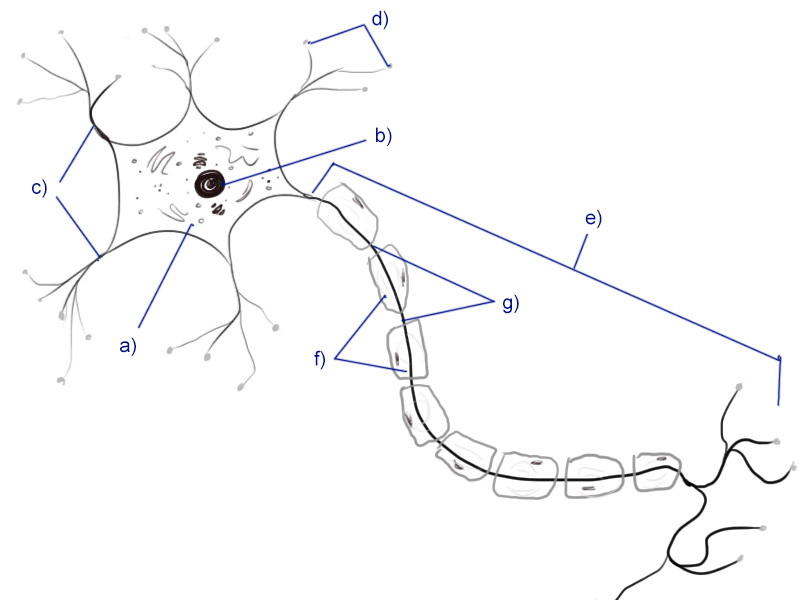
\includegraphics[width=0.7\textwidth]{img/neuron.jpg}}
		\caption{Grafika przedstawiająca schematyczną budowę neuronu na podstawie danych z ~\cite{neurology}.\\ 
		a)Soma/perykarion - ciało neuronu zawierające SER, RER, aparaty Golgiego, neurotubule i neurofilamenty, rybosomy, mitochondria, a także b) jądro komórkowe, c)dendryty, d)synapsy, e)neuryt/axon, f)osłonka mielonowa, g)przewężenia Ranviera  }
		\label{fig:neuron}
	\end{figure}
	Neuron jest jednostką morfologiczno-czynnościową układu nerwowego zbudowaną według schematu przedstawionego na  rys.~\ref{fig:neuron}. Dendryty odpowiedzialne są za przewodzenie impulsów elektrycznych pobranych przez synapsy w kierunku somy - ciała komórki nerwowej. Wyprowadzeniem impulsu zajmuje się akson - wypustka osiowa. Kierunek przebiegu jest zawsze stały  - mówi o tym prawo laryzacji dynamicznej. ~\cite{anatomy}\\ 
Przemieszczanie się impulsu elektrycznego zachodzi dzięki pompie sodowo-potasowej, która utrzymuje w komórce stałe napięcie powierzchniowe na błonie komórkowej. Potencjał spoczynkowy dla komórek nerwowych mieści się między -60, a -90mV, natomiast gdy dochodzi do pobudzenia komórki błona posiada potencjał czynnościowy, który mieści się między +20-50mV~\cite{neurology}. Właśnie dzięki postępującej różnicy potencjałów dochodzi do przewodzenia impulsu od dendrytu do aksonu i tym sposobem do kolejnego neuronu lub narządu wykonawczego.
\subsection{Podział układu nerwowego}
Układ nerwowy można podzielić najogólniej na układ somatyczny oraz autonomiczny. W skład pierwszego wchodzi ośrodkowy układ nerwowy oraz obwodowy układ nerwowy. Ośrodkowym układem nerwowym nazywa się mózgowie wraz z rdzeniem kręgowym, a obwodowym nerwy oraz zwoje. Schematyczny obraz układu nerwowego przedstawiono na rys.~\ref{fig:nervesystem} - kolorem czerwonym centralny układ nerwowy, niebieskim obwodowy układ nerwowy. Układ autonomiczny składa się z układu współczulnego i przywspółczulnego. \\
\begin{figure}[!h]

		\centering		
		 \scalebox{0.7}{
		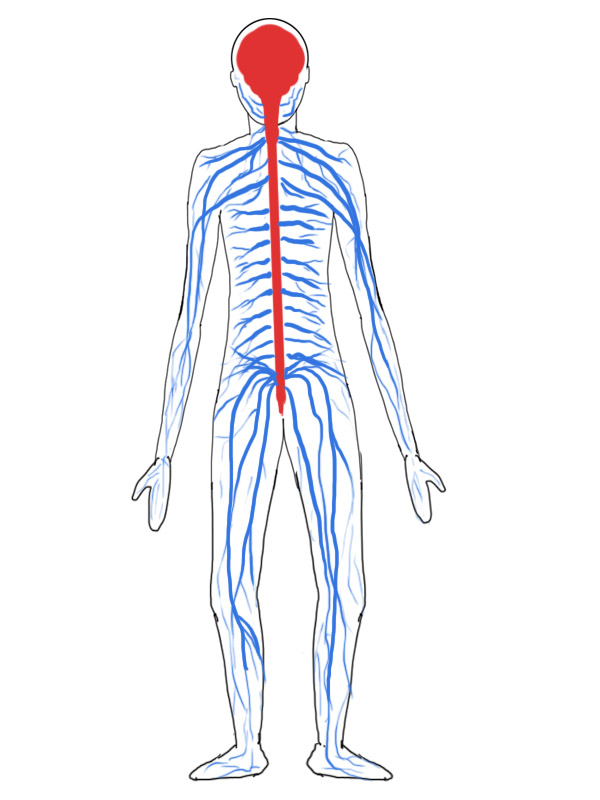
\includegraphics[width=0.7\textwidth]{img/nervesystem.jpg}}
		\caption{Grafika przedstawiająca schematyczną budowę układu nerwowego. }
		\label{fig:nervesystem}
	\end{figure}
	
Nerwy z kolei rozróżnia się ze względu na kierunek przewodnictwa na nerwy ruchowe można podzielić na ruchowe (tkzw. motoneurony) oraz czuciowe, lub też mieszane - ruchowo-czuciowe. Zgrupowanie komórek nerwowych poza ośrodkowym układem nerwowym nazywa się zwojem. 

	
	

\section{Zanikowe  stwardnienie boczne (ALS)}
\subsection{ Opis jednostki chorobowej}

Zanikowe stwardnienie boczne ( ang. amyotrophic lateral sclerosis ALS, łac. sclerosis lateralis
amyotrophica SLA) jest rzadką chorobą neurologiczną, dotyczącą  w 75\% przypadków zachorowań mężczyzn między 40 a 65 rokiem życia. ~\cite{neurology} Jednakże termin ALS jest używany do określania więcej niż jednego schorzenia związanego z degeneracją neuronów ruchowych.  Najczęściej stosowany jest, gdy mowa jest o klasycznej formie ALS (choroba Charcota), ale także w przypadku: Postępującego Porażenia Opuszkowego (Progressive bulbar palsy (PBP)), Postępującego Zaniku Mięśni (Progressive muscular atrophy (PMA)), Pierwotnego Stwardnienia Bocznego (Primary lateral sclerosis  (PLS)), Syndromu Ramienia Cepowatego (Flail arm syndrome (Vulpian-Bernhardt syndrome)), Syndromu Nogi Cepowatej (Flail leg syndrome  (Pseudopolyneuritic form)) oraz ALS  z powikłaniami wielonarządowymi  (np. ALSDementia) ~\cite{alsWij}. W celu ujednolicenia nazewnictwa Lord Russell Brain zaproponował termin Chorób Neuronu Ruchowego (Motor Neurone Disease (MND)). ~\cite{alsWij}\\
Istotą choroby jest zwyrodnienie komórek nerwowych odpowiedzialnych za przekazywanie sygnałów, wynikiem czego jest atrofia unerwianych przez nie mięśni. Degenerują neurony kory motorycznej (górny motoneuron), oraz neurony ruchowe rogów brzusznych rdzenia kręgowego, lub rdzenia przedłużonego (opuszki) (dolny motoneuron). Objawia się to początkowo ich osłabieniem, a ostatecznie zanikiem (przy czym same komórki mięśniowe nie obumierają, a jedynie zmniejszają swój rozmiar), co skutkuje ograniczeniem ruchów chorego, między innymi: gryzienia, chodzenia, mówienia i oddychania. ALS nie atakuje układu pokarmowego oraz krwionośnego. Swoją funkcjonalność stosunkowo długo zachowują neurony jądra Onufa unerwiające pęcherz moczowy i jądro nerwu okoruchowego odpowiedzialnego za ruchy gałek ocznych. Drogi czuciowe i sprawność intelektualna są zachowane. ~\cite{parkinsonALS} Powoduje to, że pacjent jest więźniem we własnym ciele - często nie mogącym się skomunikować z otoczeniem.  Co więcej ciągła świadomość pogarszającego się stanu chorego znacząco wpływa na jego samopoczucie i zdrowie psychiczne, prowadząc do depresji. \\
Nieznane są przyczyny zachorowań, jednak autorzy publikacji ~\cite{alsWij} oraz ~\cite{motoneuron} są zdania iż ALS jest wynikiem wzajemnego oddziaływania wielu czynników takich jak: czynniki genetyczne (między innymi dziedziczny defekt genu odpowiedzialnego za syntezę enzymu- desmutazy ponadtlenku Cu/Zn. [~\cite{neurology}-~\cite{alsWij}]), ekscytotoksyczność (patologiczny proces, w którym neurony są uszkadzane i zabijane przez aminokwasy o charakterze kwasowym m.in. glutaminian), stres oksydacyjny (gromadzenie reaktywnych form tlenu, na skutek zakłócenia równowagi pomiędzy ich wytwarzaniem, a biologiczną zdolnością do szybkiej detoksykacji, co prowadzi do obumierania komórek), dysfunkcje mitochondrialne (nieprawidłowości zarówno w ich budowie jak i funkcji), ograniczony transport aksonalny, anormalne gromadzenie neurofilamentów (to grupa białek włókienkowych stanowiących jeden z głównych komponentów cytoszkieletu komórek nerwowych), agregacja białek w cytoplazmie w postaci wtrętów, zaburzenia układu odpornościowego, reakcje autoimmunologiczne oraz niedobór neurotransmiterów.
ALS jest chorobą postępującą, co oznacza, że wraz z biegiem czasu następuje nasilenie objawów, w tym całkowita utrata kontroli nad ruchami dobrowolnymi. Na dzień dzisiejszy jest nieuleczalna i prowadzi do śmierci chorego w przeciągu 1-2 lat (25\% chorych). Jednak należy pamiętać, że SLA w swoim przebiegu jest chorobą bardzo indywidualną, więc tzw. okres przeżycia może wahać się w szerokich granicach. Ponad 25\% chorych przeżywa więcej niż 5 lat, w tym ok. 5\%  powyżej 10 lat .~\cite{poradnik}
\subsection{Próby terapii chorych.}

Do tej pory nie został znaleziony sposób skutecznego leczenia przyczynowego ALS. Jedynym lekiem o sprawdzonej skuteczności i dopuszczonym do stosowania w terapii  jest Rilutek (Riluzole, benzotiazol). Autorzy książki ~\cite{alsAdamek} poświęconej schorzeniu donoszą, że  „Badania  naukowe  dowodzą, że leczenie Riluzolem w dawce 100 mg dziennie (2x50 mg) przez 18 miesięcy nieznacznie  wydłuża  przeżycia  chorych  (średnio 3 – 4 miesiące)  niestety  nie  wpływając  na  poprawę  ich  stanu  klinicznego  i  jakości życia.”.  Terapia farmakologiczna chorych na ALS sprowadza się więc do leczenia objawowego.  

Innym ważnym aspektem terapii chorego jest odpowiednia rehabilitacja. Zwiększenie zakresu ruchów chorego oraz jak najdłuższe utrzymanie jego zdolności do samodzielnego wykonywania codziennych czynności jest głównym zadaniem specjalistycznej rehabilitacji ruchowej, która powinna być prowadzona od momentu diagnozy. Przykładowo wykonywane są: ćwiczenia w sali gimnastycznej, zajęcia ruchowe w basenie wzmacniające odpowiednie grupy mięśni, ćwiczenia czynne na sali chorych (chodzenie w balkonikach, stabilizatorach), czy też ćwiczenia bierne w łóżku chorego połączone z masażem leczniczym u pacjentów bez spastycznego napięcia.~\cite{alsAdamek} Korzystne efekty mogą wywoływać też takie zabiegi jak hydroterapia, kąpiele cieplne, elektroterapia, krioterapia. ~\cite{poradnik}\\
Z powodu utraty kontroli nad aparatem mowy komunikacja z chorym może stać się ograniczona, lub wręcz niemożliwa, dlatego lekarze, logopedzi i opiekunowie pacjenta mają za zadanie jak najdłuższe utrzymanie komunikacji.  Mowa tu nie tylko o komunikacji werbalnej, ale o nowych metodach wypracowywanych  indywidualnie przez chorego i opiekuna. 
Przy  narastających  zaburzeniach  dyzartrycznych  wykorzystuje  się metody  systemu  ACC  (ang.  Augmentive  and  Alternative  Communication  System)  czyli  wspomagającego  zastępczego  systemu  komunikacji,  zwiększającego możliwości komunikacyjne.~\cite{alsAdamek}

\section{Augmentative and Alternative Communication System}


Augmentative and alternative communication (AAC) jest dziedziną badań klinicznych oraz edukacyjnych. Głównym założeniem jest próba zgłębienia oraz kompensacji, gdy to konieczne, tymczasowych lub trwałych upośledzeń, czy też ograniczeń ze względu na możliwość posługiwania się oraz rozumienia komunikacji werbalnej oraz pisemnej.  Najczęstszymi przyczynami sięgania do tych metod komunikacji są: upośledzenia umysłowe, mózgowe porażenie dziecięce, autyzm oraz postępująca apraksja mowy ~\cite{augmentative} (jak w przypadku ALS). Zadaniem AAC nie jest jedynie wprowadzenie możliwości komunikacji osób chorych z otoczeniem, ale także umożliwienie im czynnego udziału w życiu społecznym oraz towarzyskim, wykonywania czynnego zawodu, czy też poświęcaniu się hobby jak pisanie prozy, bądź poezji, co w sposób znaczący odbija się na ich samopoczuciu oraz jakości życia. Dąży się zatem do zapewnienia tego podstawowego prawa każdemu pacjentowi. 


	ACC polega na wymianie wiadomości, które muszą zostać sformułowane, przechowane oraz odzyskane w dowolnym momencie. Wiadomością może być pojedyncze słowo, kod lub też struktury bardziej złożone mające na celu podtrzymanie komunikacji interpersonalnej, pisanej – także tej na mediach społecznościowych, które w dzisiejszych czasach stanowią ważny filar interakcji międzyludzkich.
\\ Istnieje kilka metod formowania pełnych zdań : jedną z nich jest wpisywanie wiadomości znak po znaku, inną jest korzystanie z gotowych bibliotek wyrazów. Możliwe jest także wykorzystanie już gotowych wzorów pełnych, lub części zdań – co zdecydowanie przyspiesza komunikację, jednak metoda ta jest ograniczona przez pamięć biblioteki przechowującej takie wzorce. Biblioteka taka tworzona i kompletowana jest zgodnie z indywidualnymi potrzebami chorego i zależy od jego płci, wieku, zawodu, stylu życia itp. Dla dzieci przygotowywane są specjalne tablice obrazkowe, które pozwalają im na jasny przekaz. \\
Tablice można podzielić ze względu na ich ułożenie obiektów na statyczne oraz dynamiczne. W tablicach statycznych każdy obiekt ma swoje ustalone położenie, które nie zmienia. Do komunikacji niezbędna jest więc duża ilość statycznych tablic – przykładem są tablice fizyczne – papierowe, gdzie nie można zmieniać położenia wydrukowanych na kartce elementów. Dynamiczne wyświetlacze odnoszą do się wyświetlaczy komputowych, w których dzięki odpowiedniemu oprogramowaniu, można dynamicznie poruszać się między widokami.  
W celu ułatwienia korzystania z bibliotek zebranych w tablice istnieje kilka metod przedstawionych w ~\cite{augmentative}.
\begin{enumerate}
\item Semantic-Syntactic Grid Displays (Semantyczno-syntaktyczna siatka/tablica) – tablica cechująca się podziałem wyświetlanych na niej słów na kategorie, zazwyczaj ze względu na części mowy. Możliwe jest także przedstawienie słów w logicznej kolejności występowania w zdaniu. Przykładowym algorytmem sortowania jest klucz Fitzgeralda – słowa układa się od lewej do prawej, układając je w klasy odpowiadające na pytania: „Kto?”, „Co robi?”, „Co?”, „Gdzie?”, „Jaki?”, „Kiedy?” itd.  Słowa, bądź litery najczęściej wybierane układane są w pierwszym bądź ostatnim wierszu tablicy. Elementem stanowczo usprawniającym korzystanie było kolorowanie elementów zgodnie z ich przynależnością do  klasy. 
\item Taxonomic Grid Displays (Siatka/tablica taksonomiczna) – dzieli słownictwo na klasy: osoby, miejsca, uczucia, jedzenie, napoje, słowa opisujące czynności. Nie jest to rekomendowany typ tablic dla dzieci w wieku poniżej 6 roku życia. 
\item Activity Grid Displays ( Tablica/siatka czynności) – najpopularniejszy typ tablic. Kategoryzacja słownictwa następuje ze względu na rodzaj czynności, wydarzenia, czy rutyny, której ono dotyczy np. „zakupy” lub „płacenie przy kasie”, czy też „rozmowa ze sprzedawcą”. Każda kategoria jest podzielona jak wyżej na mniejsze podklasy ze względu na to, co dane słowo określa. 
\item Pragmatic Organization Dynamic Display (Dynamiczny wyświetlacz  struktur pragmatycznych) – metoda kładącą duży nacisk na efektywność komunikacji, w tym celu stosując kombinację kilku różnych strategii organizacji słownictwa. 
\item Visual Scene Displays (Wyświetlacz obrazkowy) – słownictwo posortowane jest według przynależności do czynności lub rutyny, które zobrazowane są w postaci  symbolu kojarzącego się z nimi. Rozmieszczenie tych grafik nie jest siatkowe, a metodyczne. Takie rozwiązanie wykazało się wyjątkowo skuteczne w pracy z małymi dziećmi, które w bardzo krótki czasie opanowały taką formę komunikacji.  Zauważono także większą chęć interakcji w przypadku korzystania z tej formy niż w przypadku korzystania z tablic. 
\item Hybrid Display ( Wyświetlacz hybrydowy) – połączenie metody wyświetlacza obrazkowego oraz tablic. Przedstawia się zdjęcie,  na którym zaznaczone są elementy i wyświetlone związane z nimi słowa np. na obrazku widać osobę, więc wyświetlane będą np. części ciała, czynność jaka ta osoba wykonuje, emocje itp. 
 \ldots
\end{enumerate}
Ze szczególnym przypadkiem, który wymaga osobnego traktowania, mamy do czynienia w przypadku osób dorosłych z nabytą niepełnosprawnością- jak ma to miejsce w wypadku chorych na ALS. 93\% osób chorujących jest uzależniona od metod AAC .  Dorośli potrzebują więcej czasu, żeby przestawić się i przyzwyczaić się do niewerbalnej komunikacji, dlatego też zalecana im jest nauka korzystania np. z tablic od razu po diagnozie, nawet jeśli chory jest jeszcze w pełni sprawny. Zmiana stanu zdrowia w wypadku tej jednostki może nastąpić w bardzo krótkim czasie.   

\section{Technologiczne rozwiązania dla chorych na ALS}

Jak wyżej wspomniano, do rozwiązań dla chorych na ALS należą statyczne oraz dynamiczne tablice, jednak aby się nimi posługiwać należy albo opracować metodę AAC  np. dwa mrugnięcia oznaczają tak, a jedno nie, lub wykorzystać sygnały płynące z organizmu ludzkiego jako wskaźniki. Do mierzonych wartości należą m.in. impulsy elektryczne pochodzące z mózgu (mierzone za pomocą EEG), mięśni (mierzone za pomocą EMG) lub detekcja mikroruchów kończyn.~\cite{eyemouse} Ze względu na to, że technologie wykorzystujące  EEG wymagają bardzo stabilnych warunków elektromagnetycznych i są niezwykle czułe na szum, nie są optymalnymi rozwiązaniami dla chorych na ALS. Metodą bardzo dobrze się sprawdzającą, ze względu na długie zachowanie funkcjonalności gałek ocznych, jest EGT, czy też eye-tracking, czyli śledzenie wzroku. Jest to metoda bardziej niezawodna niż wyżej wymienione. 
\subsection{Eye-tracking} 

Eye-tracking, znany również jako okulorografia,  ma za zadanie np. określenie ruchów gałek ocznych, a przez to  punktu fiksacji wzroku,  najczęściej w czasie rzeczywistym. Do metod pozwalających na śledzenie wzroku oraz ruchów oczu należy m.in. elektrookulografia, śledzenie ruchu gałek ocznych, powiek, metody działające w oparciu o szkła kontaktowe, metody wykorzystujące refleksy na rogówce lub źrenicy~\cite{eyemouse}. Do poprawnego działania wymienionych metody najczęściej niezbędny jest również pomiar ruchów głowy.
\\ Technologia ta wykorzystywana jest często podczas badań marketingowych do określenia skuteczności reklamy – ustalenia, co przyciąga największą uwagę odbiorcy, bądź w celu orzeczenia poziomu użyteczności zaprojektowanego interfejsu.
Coraz częściej implementuje się dane techniki  np. w grach,  w medycynie m. in. w celu umożliwienia korzystania z urządzeń ekranowych osobom z upośledzeniami fizycznymi, które ich przed tym powstrzymują oraz wszędzie tam, gdzie użytkownik nie może mięć zajętych rąk. We współpracy z urządzeniami elektronicznymi takimi jak  komputer lub urządzenia mobilne osoba upośledzona, bądź chora może w sposób znaczący poprawić swoją jakoś życia. W celu sprawnej współpracy niezbędne jest dokładne określenie punktu fiksacji wzroku (punktu, na którym użytkownik skupia swój wzrok przez co najmniej 0,15s)~\cite{kunkaUwaga}.
\subsubsection{Podział urządzeń do eye-trackingu}

Z przykładem bardzo dobrego podziału urządzeń można zapoznać się na materiałach wykładowych pana dr inż. Bartoszka Kunki ~\cite{kunkaFiksacja}. Według niego pierwszym kryterium podziały powinna być mobilność urządzenia pomiarowego na: mobilne i niemobline, gdzie do pierwszych zaliczyć można wszystkie urządzenia nagłowne np. smartglasses, a do drugich urządzenia stacjonarne – związane na stałe np. z monitorem lub zamontowane na stojakach – mam wtedy do czynienia najczęściej z urządzeniami bezdotykowymi. Urządzenia mobilne bazują na technice wykorzystujące podczerwień, natomiast stacjonarne mogą, prócz wyżej wspomnianej, monitorować badane parametry również niezależnie od światła  IR – wykorzystując światło dzienne. 

\paragraph{Działanie urządzeń opartych na oświetleniu w podczerwieni. [~\cite{kunkaFiksacja}, ~\cite{erica}]}\leavevmode\\
W celu obserwacji ruchów gałki ocznej i określenia punktu fiksacji należy oko naświetlać światłem punktowym w podczerwieni albo w linii zgodnej z osią kamery, bądź poza nią i w zależności od wybranej metody zauważa się inne zjawiska optyczne. Podczerwień powoduje znaczy wzrost kontrastu między tęczówką, a źrenicą oka, co pozawala na dokładniejsze określenie pozycji źrenicy, co wyznaczane jest na podstawie odbicia obserwowanego na nagraniu tworzonym przez kamerę, która przez cały czas działania aparatury  skierowana jest na jedno z oczu osoby badanej~\cite{erica}.
Wśród obserwowanych odbić najbardziej istotnym względem badanego aspektu jest tzw. glint (błysk na rogówce, powstający, gdy dioda jest poza osią kamery). Glint, znany również jako  pierwszy obraz Purkinjego [~\cite{kunkaFiksacja},~\cite{erica}], nie zmienia swego położenia wraz z ruchami gałki ocznej – dlatego uważany jest jako punkt referencyjny, tak dług, jak głowa badanej osoby pozostaje nieruchoma względem kamery.  Diody umieszczone na osi kamery wywołują zjawisko jasnej źrenicy ~\cite{kunkaFiksacja} – część podczerwonego światła przedostaje się do źrenicy i zostaje od niej odbita, wywołując efekt  przypominający np. kocie oko oświetlone w ciemności.  Porównując więc pozycję glinta (lub glintów) oraz ruchomej jasnej źrenicy jesteśmy w stanie na podstawie ich względnego położenia określić punkt fiksacji oka. Określenie kierunku skierowania wzroku na podstawie względnego położenia glintu oraz źrenicy na grafice  ~\ref{fig:glint}. Schemat algorytmu wyznaczania punktu fiksacji przedstawiono na rysunku ~\ref{fig:glintUML} opartym na materiałach wykładowych ~\cite{kunkaFiksacja}.

\begin{figure}[!h]
		\centering
		\scalebox{.7}{
		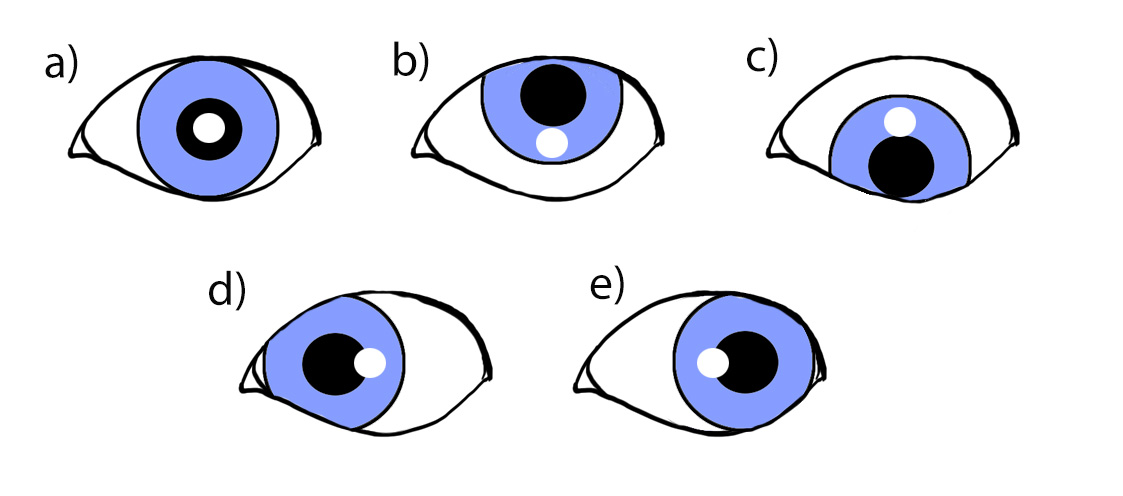
\includegraphics[width=0.7\textwidth]{img/glint.jpg}}
		\caption{Położenie glinta względem środka źrenicy w zależności od ruchu gałki ocznej. \\
a) patrzenie prosto w źródło światła b) patrzenie powyżej źródła światła c) patrzenie poniżej źródła światła d)patrzenie w lewo od źródła światła e)patrzenie w prawo od źródła światła 
}
		\label{fig:glint}
	\end{figure}
	
\begin{figure}[!h]

		\centering		
		 \scalebox{.65}{
		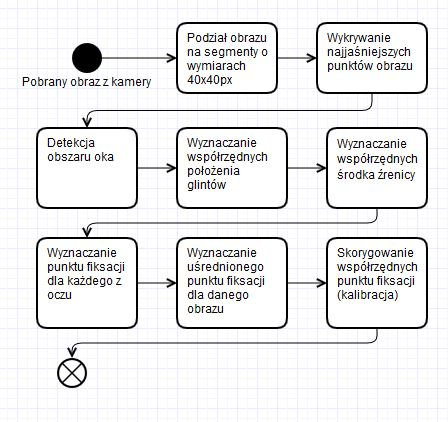
\includegraphics[width=0.7\textwidth]{img/UMLglint.JPG}}
		\caption{Poglądowy schemat algorytmu wyznaczania punktu fiksacji przy wykorzystaniu światła IR. }
		\label{fig:glintUML}
	\end{figure}
	
Odległości wyliczane są  na postawie obrazów przechwyconych  przez kamerę i przetworzonych komputerowo.  
Tą samą technologię można również zmodyfikować, by wyznaczać punkt fiksacji  z położenia 4 glintów ( wywołanych 4 diodami rozmieszczonymi w narożnikach ekranu) lub przy zastosowaniu skomplikowanych  przekształceń matematycznych,  poprawiających dokładność  wyznaczenia punktu fiksacji. ~\cite{kunkaFiksacja}
Inną metodą – wykorzystującą  na przemian dwa rodzaje diod ( na lub poza osią kamery) jest metoda różnicowa ~\cite{kunkaFiksacja}. Wykorzystuje się kolejne klatki nagrania, przy czym jedna klatka zawiera efekt jasnej źrenicy, a druga zawiera efekt ciemnej źrenicy i glinty. Punkt fiksacji po raz kolejny jest wynikiem różnicy odległości obu zjawisk i obliczany jest na podstawie wynikowego obrazu różnicowego.\\
Przykładami technologii, które do tej pory wykorzystały powyższy algorytm to np. Erica[1989].
\paragraph{Działanie urządzeń  opartych na świetle dziennym. }\leavevmode\\
W przypadku  metod  wykorzystujących światło dzienne i kamerę rejestrujące ruchy gałek ocznych mamy do czynienia z bardzo złożonymi algorytmami komputerowymi, które pozwalają na przetwarzania obrazu powodującego określenie punktu fiksacji wzroku. Wraz z zaletą, jaką jest brak zapotrzebowanie na dodatkowy sprzęt (algorytmy mogą współpracować z wbudowanymi kamerkami komputerowymi), technologie te niestety często charakteryzują się gorszą dokładnością.

Przykładem technologii korzystającej ze światła dziennego jest Eye Mouse – projekt powstały na terenie Politechniki Gdańskiej ~\cite{eyemouse}, którego głównym założeniem jest wykorzystanie wzroku jako zastępstwo myszy komputerowej oraz klawiatury.W tym celu wykorzystuje się dwie kamery – jednej śledzącej wzrok, a drugiej położenie głowy osoby badanej względem ekranu – tak, że na otrzymywany wynik nanoszona jest korekta.  W rogach ekranu umieszczone są 4 diody światła podczerwonego jako znaczniki. W procesie przetwarzania obrazów usuwany jest szum oraz wyznaczana jest źrenica oraz jej środek. Kolejnym krokiem jest oznaczenie wzajemnej zależności pozycji ekranu względem głowy osoby badanej – w tym celu wykorzystuje się znaczniki LED. Proces ten niezbędny jest w celu kalibracji.
\section{Podsumowanie}
Zapoznawszy się z problematyką choroby zanikowego stwardnienia bocznego oraz z możliwościami technologicznymi oferowanymi pacjentom można przejść do stworzenia aplikacji komputerowej, która ma za cel ułatwienie komunikacji chorych z komputerem. Wykorzysta się do tego metodę eye-trackingu korzystającej ze światła dziennego - zwiększając w ten sposób dostępność oraz uniwersalność aplikacji. 

\end{document}


\documentclass[twoside,a4paper]{book}
\usepackage{graphicx}
\usepackage{hyperref}
\usepackage{amsmath}
\usepackage{amssymb}
\usepackage{textcomp}
\usepackage[utf8]{inputenc}
\usepackage[polish]{babel}
\usepackage[T1]{fontenc}
\usepackage{standalone}
\usepackage{array}
% pakiet stosowany do url'i w bibliografii, zamienia odnośniki na ładnie sformatowane
\usepackage{url}
% pakiety służące do numerowania i tworzenia algorytmów
\usepackage{algorithmic}
\usepackage{algorithm}
% redefinicja etykiety nagłówkowej listy algorytmów, domyślna jest po angielsku
\renewcommand{\listalgorithmname}{Spis algorytmów}

\usepackage[section]{placeins}
\usepackage{pdfpages}

% pakiet do wyliczania skali, przydatny przy dużych obrazkach
\usepackage{pgf}
% pakiet służący do automatycznego sortowania odnośników do bibliografii
\usepackage[sort]{natbib}
% tworzenie listingów
\usepackage{listings}
% tworzenie figur wewnątrz figur
\usepackage{subfig}
% do automatycznego skracania nazw rozdziałów i podrozdziałów używanych w nagłówkach strony by mieściły się w jednej linii
\usepackage[fit]{truncate}
% fancyhdr - ładne nagłówki, definicja wyglądu nagłówka, numery stron będą umieszczane w nagłówku po odpowiedniej stronie
\usepackage{fancyhdr}
\pagestyle{fancy}
\renewcommand{\chaptermark}[1]{\markboth{#1}{}}
\renewcommand{\sectionmark}[1]{\markright{\thesection\ #1}}



\fancyhf{}
\fancyhead[LE,RO]{\bfseries\thepage}
% tutaj ograniczamy szerokość pola w nagłówku zawierającego nazwę rozdziału/podrozdziału do 95% szerokości strony
% redefinicja sposobu prezentacji nazw domyślnie wypisywanych wielkimi literami (np. domyślnie w nagłówku Spis treści będzie miał postać SPIS TREŚCI)
% Uwaga! to może popsuć wielkie litery w ogóle! Jak coś nie działa należy usunąć \nouppercase{} z poniższych definicji
\fancyhead[LO]{\nouppercase{\bfseries{\truncate{.95\headwidth}{\rightmark}}}}
\fancyhead[RE]{\nouppercase{\bfseries{\truncate{.95\headwidth}{\leftmark}}}}
\renewcommand{\headrulewidth}{0.5pt}
\renewcommand{\footrulewidth}{0pt}

% definicja typu prostego wymagana przez pierwsze strony rozdziałów itp.
% powyższe reguły niestety tych stron nie dotyczą, gdyż Latex automatycznie przełącza je pomiędzy fancy a plain
% w tym wypadku eliminujemy nagłówki i stopki na stronach początkowych
\fancypagestyle{plain}{%
 \fancyhead{}
 \fancyfoot{}
 \renewcommand{\headrulewidth}{0pt}
 \renewcommand{\footrulewidth}{0pt}
}

\parskip 0.05in


% makro umożliwiające otaczanie symboli okręgami
\usepackage{tikz}
% brak justowania tekstu (bazą okręgu będzie linia tekstu)
\newcommand*\mycirc[1]{%
  \begin{tikzpicture}
    \node[draw,circle,inner sep=1pt] {#1};
  \end{tikzpicture}}

% pionowe justowanie tekstu, środek okręgu pokrywa się ze środkiem tekstu
\newcommand*\mycircalign[1]{%
  \begin{tikzpicture}[baseline=(C.base)]
    \node[draw,circle,inner sep=1pt](C) {#1};
  \end{tikzpicture}}

% zmiana nazwy twierdzeń i lematów
\newtheorem{theorem}{Twierdzenie}[section]
\newtheorem{lemma}[theorem]{Lemat}

% tworzenie definicji dowodu
\newenvironment{proof}[1][Dowód]{\begin{trivlist}
\item[\hskip \labelsep {\bfseries #1}]}{\end{trivlist}}
% \newenvironment{definition}[1][Definicja]{\begin{trivlist}
% \item[\hskip \labelsep {\bfseries #1}]}{\end{trivlist}}
% \newenvironment{example}[1][Przykład]{\begin{trivlist}
% \item[\hskip \labelsep {\bfseries #1}]}{\end{trivlist}}
% \newenvironment{remark}[1][Uwaga]{\begin{trivlist}
% \item[\hskip \labelsep {\bfseries #1}]}{\end{trivlist}}

% definicja czarnego prostokąta zwyczajowo dodawanego na koniec dowodu
\newcommand{\qed}{\nobreak \ifvmode \relax \else
      \ifdim\lastskip<1.5em \hskip-\lastskip
      \hskip1.5em plus0em minus0.5em \fi \nobreak
      \vrule height0.75em width0.5em depth0.25em\fi}

% poniższymi instrukcjami można sterować co ma być numerowane a co nie i co ma być wyświetlane w spisie treści
% \setcounter{secnumdepth}{3}
% \setcounter{tocdepth}{5}

% definicja czcionki mniejszej niż tiny (domyślnie takiej małej nie ma)
\usepackage{lmodern}
\makeatletter
  \newcommand\tinyv{\@setfontsize\tinyv{4pt}{6}}
\makeatother

% definicja jeszcze mniejszej czcionki
\usepackage{lmodern}
\makeatletter
  \newcommand\tinyvv{\@setfontsize\tinyvv{3.5pt}{6}}
\makeatother

% pakiet do obsługi wielostronicowych tabel
\usepackage{longtable}
\setlength{\LTcapwidth}{\textwidth}

\usepackage[section] {placeins}

\usepackage{multirow}

\usepackage{slantsc}
\usepackage[labelsep=endash]{caption}
\addto\captionspolish{\renewcommand{\figurename}{Rys.}}
\addto\captionspolish{\renewcommand{\tablename}{Tab.}}
\addto\captionspolish{\renewcommand*{\appendixpagename}{Dodatki}}
\addto\captionspolish{\renewcommand*{\appendixtocname}{Dodatki}}
\addto\captionspolish{\renewcommand*{\appendixname}{Dodatek}}

\setcounter{secnumdepth}{5}

\usepackage[toc,page]{appendix}

\begin{document}
\chapter{Stan wiedzy}
\section{Układ nerwowy}
\section{Zanikowe  stwardnienie boczne (ALS)}
\subsection{ Opis jednostki chorobowej}

Zanikowe stwardnienie boczne ( ang. amyotrophic lateral sclerosis ALS, łac. sclerosis lateralis
amyotrophica SLA) jest rzadką chorobą neurologiczną, dotyczącą  w 75\% przypadków zachorowań mężczyzn między 40 a 65 rokiem życia. ~\cite{neurology} Jednakże termin ALS jest używany do określania więcej niż jednego schorzenia związanego z degeneracją neuronów ruchowych.  Najczęściej stosowany jest, gdy mowa jest o klasycznej formie ALS (choroba Charcota), ale także w przypadku: Postępującego Porażenia Opuszkowego (Progressive bulbar palsy (PBP)), Postępującego Zaniku Mięśni (Progressive muscular atrophy (PMA)), Pierwotne Stwardnienie Boczne (Primary lateral sclerosis  (PLS)),Syndrom Ramienia Cepowatego (Flail arm syndrome (Vulpian-Bernhardt syndrome)),  Syndrom Nogi Cepowatej (Flail leg syndrome  (Pseudopolyneuritic form)) oraz ALS  z powikłaniami wielonarządowymi  (np. ALSDementia) ~\cite{alsWij}.W celu ujednolicenia nazewnictwa Lord Russell Brain zaproponował termin Chorób Neuronu Ruchowego (Motor Neurone Disease (MND)). ~\cite{alsWij}\\
Istotą choroby jest zwyrodnienie komórek nerwowych (Degenerują neurony kory motorycznej (górny motoneuron), oraz neurony ruchowe rogów brzusznych rdzenia kręgowego, lub rdzenia przedłużonego (opuszki) (dolny motoneuron)) odpowiedzialnych za przekazywanie sygnałów, wynikiem czego jest atrofia unerwianych przez nie mięśni. Objawia się to początkowo ich osłabieniem, a ostatecznie zanikiem (przy czym same komórki mięśniowe nie obumierają, a jedynie zmniejszają swój rozmiar), co skutkuje ograniczeniem ruchów chorego, między innymi: gryzienia, chodzenia, mówienia i oddychania. ALS nie atakuje układu pokarmowego oraz krwionośnego. Swoją funkcjonalność stosunkowo długo zachowują neurony jądra Onufa unerwiające pęcherz moczowy i jądro nerwu okoruchowego odpowiedzialnego za ruchy gałek ocznych. Drogi czuciowe i sprawność intelektualna są zachowane. ~\cite{parkinsonALS} Powoduje to, że pacjent jest więźniem we własnym ciele - często nie mogącym się skomunikować z otoczeniem.  Co więcej ciągła świadomość pogarszającego się stanu chorego znacząco wpływa na jego samopoczucie i zdrowie psychiczne, prowadząc do depresji. \\
Nieznane są przyczyny zachorowań, jednak autorzy publikacji ~\cite{alsWij} są zdania iż ALS jest wynikiem wzajemnego oddziaływania wielu czynników takich jak: czynniki genetyczne (między innymi dziedziczny defekt genu odpowiedzialnego za syntezę enzymu- desmutazy ponadtlenku Cu/Zn. [~\cite{neurology}-~\cite{alsWij}]), ekscytotoksyczność (patologiczny proces, w którym neurony są uszkadzane i zabijane przez aminokwasy o charakterze kwasowym m.in. glutaminian), stres oksydacyjny (gromadzenie reaktywnych form tlenu, na skutek zakłócenia równowagi pomiędzy ich wytwarzaniem, a biologiczną zdolnością do szybkiej detoksykacji, co prowadzi do obumierania komórek), dysfunkcje mitochondrialne (nieprawidłowości zarówno w ich budowie jak i funkcji), ograniczony transport aksonalny, anormalne gromadzenie neurofilamentów (to grupa białek włókienkowych stanowiących jeden z głównych komponentów cytoszkieletu komórek nerwowych), agregacja białek w cytoplazmie w postaci wtrętów, zaburzenia układu odpornościowego, reakcje autoimmunologiczne oraz niedobór neurotransmiterów.
ALS jest chorobą postępującą, co oznacza, że wraz z biegiem czasu następuje nasilenie objawów, w tym całkowita utrata kontroli nad ruchami dobrowolnymi. Na dzień dzisiejszy jest nieuleczalna i prowadzi do śmierci chorego w przeciągu 1-2 lat (25\% chorych). Jednak należy pamiętać, że SLA w swoim przebiegu jest chorobą bardzo indywidualną, więc tzw. okres przeżycia może wahać się w szerokich granicach. Ponad 25\% chorych przeżywa więcej niż 5lat, w tym ok. 5\%  powyżej 10 lat .~\cite{poradnik}
\subsection{Próby terapii chorych.}

Do tej pory nie został znaleziony sposób skutecznego leczenia przyczynowego ALS. Jedynym lekiem o sprawdzonej skuteczności i dopuszczonym do stosowania w terapii  jest Rilutek (Riluzole, benzotiazol). Autorzy książki ~\cite{alsAdamek} poświęconej schorzeniu donoszą, że  „Badania  naukowe  dowodzą, że leczenie Riluzolem w dawce 100 mg dziennie (2x50 mg) przez 18 miesięcy nieznacznie  wydłuża  przeżycia  chorych  (średnio 3 – 4 miesiące)  niestety  nie  wpływając  na  poprawę  ich  stanu  klinicznego  i  jakości życia.”.  Terapia farmakologiczna chorych na ALS sprowadza się więc do leczenia objawowego.  


Innym ważnym aspektem terapii chorego jest odpowiednia rehabilitacja. Zwiększenie zakresu ruchów chorego oraz jak najdłuższe utrzymanie jego zdolności do samodzielnego wykonywania codziennych czynności jest głównym zadaniem specjalistycznej rehabilitacji ruchowej, która powinna być prowadzona od momentu diagnozy. Przykładowo wykonywane są: ćwiczenia w sali gimnastycznej, zajęcia ruchowe w basenie wzmacniające odpowiednie grupy mięśni, ćwiczenia czynne na sali chorych (chodzenie w balkonikach, stabilizatorach), czy też ćwiczenia bierne w łóżku chorego połączone z masażem leczniczym u pacjentów bez spastycznego napięcia.~\cite{alsAdamek} Korzystne efekty mogą wywoływać też takie zabiegi jak hydroterapia, kąpiele cieplne, elektroterapia, krioterapia. ~\cite{poradnik}\\
Z powodu utraty kontroli nad aparatem mowy komunikacja z chorym może stać się ograniczona, lub wręcz niemożliwa, dlatego lekarze, logopedzi i opiekunowie pacjenta mają za zadanie jak najdłuższe utrzymanie komunikacji.  Mowa tu nie tylko o komunikacji werbalnej, ale o nowych metodach wypracowywanych  indywidualnie przez chorego i opiekuna. 
Przy  narastających  zaburzeniach  dyzartrycznych  wykorzystuje  się metody  systemu  ACC  (ang.  Augmentive  and  Alternative  Communication  System)  czyli  wspomagającego  zastępczego  systemu  komunikacji,  zwiększającego możliwości komunikacyjne.~\cite{alsAdamek}

\subsection{Augmentative and Alternative Communication System}


Augmentative and alternative communication (AAC) jest dziedziną badań klinicznych oraz edukacyjnych. Głównym założeniem jest próba zgłębienia oraz kompensacji, gdy to konieczne, tymczasowych lub trwałych upośledzeń, czy też ograniczeń ze względu na możliwość posługiwania się oraz rozumienia komunikacji werbalnej oraz pisemnej.  Najczęstszymi przyczynami sięgania do tych metod komunikacji są: upośledzenia umysłowe, mózgowe porażenie dziecięce, autyzm oraz postępująca apraksja mowy ~\cite{augmentative} (jak w przypadku ALS). Zadaniem AAC nie jest jedynie wprowadzenie możliwości komunikacji osób chorych z otoczeniem, ale także umożliwienie im czynny udział w życiu społecznym oraz towarzyskim, wykonywanie czynne zawodu, czy też poświęcaniu się hobby jak pisanie prozy, bądź poezji, co w sposób znaczący odbija się na ich samopoczuciu oraz jakości życia. Dąży się zatem do zapewnienia tego podstawowego prawa każdemu pacjentowi. 


	ACC polega na wymianie wiadomości, które muszą zostać sformułowane, przechowane oraz odzyskane w dowolnym momencie. Wiadomością może być pojedyncze słowo, kod lub też struktury bardziej złożone mające na celu podtrzymanie komunikacji interpersonalnej, pisanej – także tej na mediach społecznościowych, które w dzisiejszych czasach stanowią ważny filar interakcji międzyludzkich. Istnieje kilka metod formowania pełnych zdań : jedną z nich jest wpisywanie wiadomości znak po znaku, inną jest korzystanie z gotowych bibliotek wyrazów. Możliwe jest także wykorzystanie już gotowych wzorów pełnych, lub części zdań – co zdecydowanie przyspiesza komunikację, jednak ograniczona jest przez pamięć biblioteki przechowującej takie wzorce. Biblioteka taka tworzona i kompletowana jest zgodnie z indywidualnymi potrzebami chorego i zależy od jego płci, wieku, zawodu, stylu życia itp. Dla dzieci przygotowywane są specjalne tablice obrazkowe, które pozwalają im na jasny przekaz. \\
Tablice można podzielić ze względu na ich ułożenie obiektów na statyczne oraz dynamiczne. W tablicach statycznych każdy obiekt ma swoje ustalone położenie, którego nie zmienia. Do komunikacji niezbędna jest więc duża ilość statycznych tablic – przykładem są tablice fizyczne – papierowe, gdzie nie możemy zmieniać położenia wydrukowanych na kartce elementów. Dynamiczne wyświetlacze odnoszą do się wyświetlaczy komputowych, w których dzięki odpowiedniemu oprogramowaniu, możemy dynamicznie poruszać się między widokami.  
W celu ułatwienia korzystania z bibliotek zebranych w tablice istnieje kilka metod przedstawionych w ~\cite{augmentative}.
\begin{enumerate}
\item Semantic-Syntactic Grid Displays (Semantyczno-syntaktyczna siatka/tablica) – tablica cechująca się podziałem wyświetlanych na niej słów na kategorie, zazwyczaj ze względu na części mowy. Możliwe jest także przedstawienie słów w logicznej kolejności występowania w zdaniu. Przykładowym algorytmem sortowania jest klucz Fitzgeralda – słowa układa się od lewej do prawej, układając je w klasy odpowiadające na pytania: „Kto?”, „Co robi?”, „Co?”, „Gdzie?”, „Jaki?”, „Kiedy?” itd.  Słowa, bądź litery najczęściej wybierane układane są w pierwszym bądź ostatnim wierszu tablicy. Elementem stanowczo usprawniającym korzystanie było kolorowanie elementów zgodnie z ich przynależnością do  klasy. 
\item Taxonomic Grid Displays (Siatka/tablica taksonomiczna) – dzieli słownictwo na klasy: osoby, miejsca, uczucia, jedzenie, napoje, słowa opisujące czynności. Nie jest to rekomendowany typ tablic dla dzieci w wieku poniżej 6 roku życia. 
\item Activity Grid Displays ( Tablica/siatka czynności) – najpopularniejszy typ tablic. Kategoryzacja słownictwa następuje ze względu na rodzaj czynności, wydarzenia, czy rutyny, której ono dotyczy np. „zakupy” lub „płacenie przy kasie”, czy też „rozmowa ze sprzedawcą”. Każda kategoria jest podzielona jak wyżej na mniejsze podklasy ze względu na to, co dane słowo określa. 
\item Pragmatic Organization Dynamic Display (Dynamiczny wyświetlacz  struktur pragmatycznych) – metoda kładącą duży nacisk na efektywność komunikacji, w tym celu stosując kombinację kilku różnych strategii organizacji słownictwa. 
\item Visual Scene Displays (Wyświetlacz obrazkowy) – słownictwo posortowane jest według przynależności do czynności lub rutyny, które zobrazowane są w postaci  symbolu kojarzącego się z nimi. Rozmieszczenie tych grafik nie jest siatkowe, a metodyczne. Takie rozwiązanie wykazało się wyjątkowo skuteczne w pracy z małymi dziećmi, które w bardzo krótki czasie opanowały taką formę komunikacji.  Zauważono także większą chęć interakcji w przypadku korzystania z tej formy niż w przypadku korzystania z tablic. 
\item Hybrid Display ( Wyświetlacz hybrydowy) – połączenie metody wyświetlacza obrazkowego oraz tablic. Przedstawia się zdjęcie,  na którym zaznaczone są elementy i wyświetlone związane z nimi słowa np. na obrazku widać osobę, więc wyświetlane będą np. części ciała, czynność jaka ta osoba wykonuje, emocje itp. 
 \ldots
\end{enumerate}
Ze szczególnym przypadkiem, który wymaga osobnego traktowania, mamy do czynienia w przypadku osób dorosłych z nabytą niepełnosprawnością- jak ma to miejsce w wypadku chorych na ALS. 93\% osób chorujących jest uzależniona od metod AAC .  Dorośli potrzebują więcej czasu, żeby przestawić się i przyzwyczaić się do niewerbalnej komunikacji, dlatego też zalecana im jest nauka korzystania np. z tablic od razu po diagnozie, nawet jeśli chory jest jeszcze w pełni sprawny. Zmiana stanu zdrowia w wypadku tej jednostki może nastąpić w bardzo krótkim czasie.   

\subsection{Technologiczne rozwiązania dla chorych na ALS}

Jak wyżej wspomniano do rozwiązań dla chorych na ALS należą statyczne oraz dynamiczne tablice, jednak aby się nimi posługiwać należy albo opracować metodę AAC  np. dwa mrugnięcia oznaczają tak, a jedno nie, lub wykorzystać sygnały płynące z organizmu ludzkiego jako wskaźniki. Do mierzonych wartości należą m.in. impulsy elektryczne pochodzące z mózgu (mierzone za pomocą EEG), mięśni (mierzone za pomocą EMG) lub detekcja mikro ruchów kończyn.~\cite{eyemouse} W przypadku pacjentów chorych na ALS metodą bardzo dobrze się sprawdzającą, ze względu na zachowanie funkcjonalności gałek ocznych, jest EGT, czyli śledzenie wzroku – obsługa oprogramowania za pomocą wzroku. Jest to metoda bardziej niezawodna niż wyżej wymienione. 

\subsubsection{Eye-tracking} 

Eye-tracking, znany również jako okulorografia,  ma za zadanie określenie ruchów gałek ocznych oraz  punktu fiksacji wzroku,  najczęściej w czasie rzeczywistym. Technologia ta wykorzystywana jest często podczas badań marketingowych do określenia skuteczności reklamy – ustalenia, co przyciąga największą uwagę odbiorcy, bądź w celu orzeczenia poziomu użyteczności zaprojektowanego interfejsu.
Coraz częściej implementuje się dane techniki  np. w grach,  w medycynie m. in. w celu umożliwienia korzystania z urządzeń ekranowych osobom z upośledzeniami fizycznymi, które ich przed tym powstrzymują oraz wszędzie tam, gdzie użytkownik nie może mięć zajętych rąk. We współpracy z urządzeniami elektronicznymi takimi jak  komputer lub urządzenia mobilne osoba upośledzona, bądź chora może w sposób znaczący poprawić swoją jakoś życia. W celu sprawnej współpracy niezbędne jest dokładne określenie punktu fiksacji wzroku (punktu, na którym użytkownik skupia swój wzrok przez co najmniej 0,15s)~\cite{kunkaUwaga}. 
\paragraph{Podział urządzeń do eye-trackingu}


Z przykładem bardzo dobrego podziału urządzeń można zapoznać się na materiałach wykładowych pana dr inż. Bartoszka Kunki ~\cite{kunkaFiksacja}. Według niego pierwszym kryterium podziały powinna być mobilność urządzenia pomiarowego na: mobilne i niemobline, gdzie do pierwszych zaliczyć można wszystkie urządzenia nagłowne np. smartglasses, a do drugich urządzenia stacjonarne – związane na stałe np. z monitorem lub zamontowane na stojakach – mam wtedy do czynienia najczęściej z urządzeniami bezdotykowymi. Urządzenia mobilne bazują na technice wykorzystujące podczerwień, natomiast stacjonarne mogą, prócz wyżej wspomnianej, monitorować badane parametry również niezależnie od światła  IR – wykorzystując światło dzienne. 
\subparagraph{Działanie urządzeń opartych na oświetleniu w podczerwieni. [~\cite{kunkaFiksacja}, ~\cite{erica}]}
W celu obserwacji ruchów gałki ocznej i określenia punktu fiksacji należy oko naświetlać światłem punktowym w podczerwieni albo w linii zgodnej z osią kamery, bądź poza nią i w zależności od wybranej metody zauważa się inne zjawiska optyczne. Podczerwień powoduje znaczy wzrost kontrastu między tęczówką, a źrenicą oka, co pozawala na dokładniejsze określenie pozycji źrenicy, co wyznaczane jest na podstawie odbicia obserwowanego na nagraniu tworzonym przez kamerę, która przez cały czas działania aparatury  skierowana jest na jedno z oczu osoby badanej~\cite{erica}.
Wśród obserwowanych odbić najbardziej istotnym względem badanego aspektu jest tzw. glint (błysk na rogówce, powstający, gdy dioda jest poza osią kamery). Glint, znany również jako  pierwszy obraz Purkinjego [~\cite{kunkaFiksacja},~\cite{erica}], nie zmienia swego położenia wraz z ruchami gałki ocznej – dlatego uważany jest jako punkt referencyjny, tak dług, jak głowa badanej osoby pozostaje nieruchoma względem kamery.  Diody umieszczone na osi kamery wywołują zjawisko jasnej źrenicy[10] – część podczerwonego światła przedostaje się do źrenicy i zostaje od niej odbita, wywołując efekt  przypominający np. kocie oko oświetlone w ciemności.  Porównując więc pozycję glinta (lub glintów) oraz ruchomej jasnej źrenicy jesteśmy w stanie na podstawie ich względnego położenia określić punkt fiksacji oka. Orientacyjny sposób wyznaczania punktu fiksacji przedstawiono na rysunku ~\ref{fig:glint}.

\begin{figure}[!h]
		\centering
		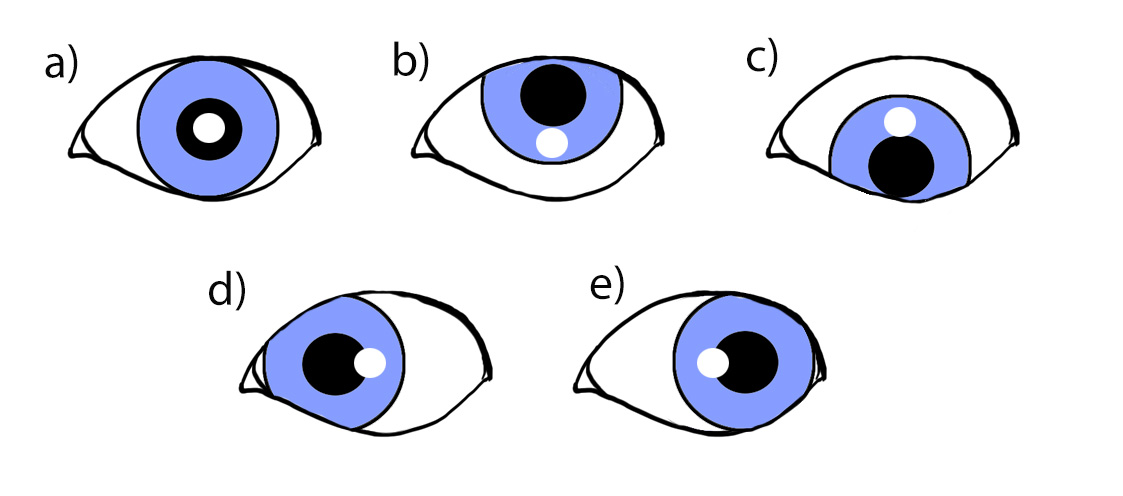
\includegraphics[width=0.7\textwidth]{img/glint.jpg}
		\caption{Położenie glinta względem środka źrenicy w zależności od ruchu gałki ocznej. \\
a) patrzenie prosto w źródło światła b) patrzenie powyżej źródła światła c) patrzenie poniżej źródła światła d)patrzenie w lewo od źródła światła e)patrzenie w prawo od źródła światła 
}
		\label{fig:glint}
	\end{figure}
	
Odległości wyliczane są  na postawie obrazów przechwyconych  przez kamerę i przetworzonych komputerowo.  
Tą samą technologię można również zmodyfikować, by wyznaczać punkt fiksacji  z położenia 4 glintów ( wywołanych 4 diodami rozmieszczonymi w narożnikach ekranu) lub przy zastosowaniu skomplikowanych  przekształceń matematycznych,  poprawiających dokładność  wyznaczenia punktu fiksacji. [10] 
Inną metodą – wykorzystującą  na przemian dwa rodzaje diod ( na lub poza osią kamery) jest metoda różnicowa [10]. Wykorzystuje się kolejne klatki nagrania, przy czym jedna klatka zawiera efekt jasnej źrenicy, a druga zawiera efekt ciemnej źrenicy i glinty. Punkt fiksacji po raz kolejny jest wynikiem różnicy odległości obu zjawisk i obliczany jest na podstawie wynikowego obrazu różnicowego.\\
Przykładami technologii, które do tej pory wykorzystały powyższy algorytm to np. Erica[1989].
\end{document}


\documentclass[twoside,a4paper]{book}
\usepackage{graphicx}
\usepackage{hyperref}
\usepackage{amsmath}
\usepackage{amssymb}
\usepackage{textcomp}
\usepackage[utf8]{inputenc}
\usepackage[polish]{babel}
\usepackage[T1]{fontenc}
\usepackage{standalone}
\usepackage{array}
% pakiet stosowany do url'i w bibliografii, zamienia odnośniki na ładnie sformatowane
\usepackage{url}
% pakiety służące do numerowania i tworzenia algorytmów
\usepackage{algorithmic}
\usepackage{algorithm}
% redefinicja etykiety nagłówkowej listy algorytmów, domyślna jest po angielsku
\renewcommand{\listalgorithmname}{Spis algorytmów}

\usepackage[section]{placeins}
\usepackage{pdfpages}

% pakiet do wyliczania skali, przydatny przy dużych obrazkach
\usepackage{pgf}
% pakiet służący do automatycznego sortowania odnośników do bibliografii
\usepackage[sort]{natbib}
% tworzenie listingów
\usepackage{listings}
% tworzenie figur wewnątrz figur
\usepackage{subfig}
% do automatycznego skracania nazw rozdziałów i podrozdziałów używanych w nagłówkach strony by mieściły się w jednej linii
\usepackage[fit]{truncate}
% fancyhdr - ładne nagłówki, definicja wyglądu nagłówka, numery stron będą umieszczane w nagłówku po odpowiedniej stronie
\usepackage{fancyhdr}
\pagestyle{fancy}
\renewcommand{\chaptermark}[1]{\markboth{#1}{}}
\renewcommand{\sectionmark}[1]{\markright{\thesection\ #1}}



\fancyhf{}
\fancyhead[LE,RO]{\bfseries\thepage}
% tutaj ograniczamy szerokość pola w nagłówku zawierającego nazwę rozdziału/podrozdziału do 95% szerokości strony
% redefinicja sposobu prezentacji nazw domyślnie wypisywanych wielkimi literami (np. domyślnie w nagłówku Spis treści będzie miał postać SPIS TREŚCI)
% Uwaga! to może popsuć wielkie litery w ogóle! Jak coś nie działa należy usunąć \nouppercase{} z poniższych definicji
\fancyhead[LO]{\nouppercase{\bfseries{\truncate{.95\headwidth}{\rightmark}}}}
\fancyhead[RE]{\nouppercase{\bfseries{\truncate{.95\headwidth}{\leftmark}}}}
\renewcommand{\headrulewidth}{0.5pt}
\renewcommand{\footrulewidth}{0pt}

% definicja typu prostego wymagana przez pierwsze strony rozdziałów itp.
% powyższe reguły niestety tych stron nie dotyczą, gdyż Latex automatycznie przełącza je pomiędzy fancy a plain
% w tym wypadku eliminujemy nagłówki i stopki na stronach początkowych
\fancypagestyle{plain}{%
 \fancyhead{}
 \fancyfoot{}
 \renewcommand{\headrulewidth}{0pt}
 \renewcommand{\footrulewidth}{0pt}
}

\parskip 0.05in


% makro umożliwiające otaczanie symboli okręgami
\usepackage{tikz}
% brak justowania tekstu (bazą okręgu będzie linia tekstu)
\newcommand*\mycirc[1]{%
  \begin{tikzpicture}
    \node[draw,circle,inner sep=1pt] {#1};
  \end{tikzpicture}}

% pionowe justowanie tekstu, środek okręgu pokrywa się ze środkiem tekstu
\newcommand*\mycircalign[1]{%
  \begin{tikzpicture}[baseline=(C.base)]
    \node[draw,circle,inner sep=1pt](C) {#1};
  \end{tikzpicture}}

% zmiana nazwy twierdzeń i lematów
\newtheorem{theorem}{Twierdzenie}[section]
\newtheorem{lemma}[theorem]{Lemat}

% tworzenie definicji dowodu
\newenvironment{proof}[1][Dowód]{\begin{trivlist}
\item[\hskip \labelsep {\bfseries #1}]}{\end{trivlist}}
% \newenvironment{definition}[1][Definicja]{\begin{trivlist}
% \item[\hskip \labelsep {\bfseries #1}]}{\end{trivlist}}
% \newenvironment{example}[1][Przykład]{\begin{trivlist}
% \item[\hskip \labelsep {\bfseries #1}]}{\end{trivlist}}
% \newenvironment{remark}[1][Uwaga]{\begin{trivlist}
% \item[\hskip \labelsep {\bfseries #1}]}{\end{trivlist}}

% definicja czarnego prostokąta zwyczajowo dodawanego na koniec dowodu
\newcommand{\qed}{\nobreak \ifvmode \relax \else
      \ifdim\lastskip<1.5em \hskip-\lastskip
      \hskip1.5em plus0em minus0.5em \fi \nobreak
      \vrule height0.75em width0.5em depth0.25em\fi}

% poniższymi instrukcjami można sterować co ma być numerowane a co nie i co ma być wyświetlane w spisie treści
% \setcounter{secnumdepth}{3}
% \setcounter{tocdepth}{5}

% definicja czcionki mniejszej niż tiny (domyślnie takiej małej nie ma)
\usepackage{lmodern}
\makeatletter
  \newcommand\tinyv{\@setfontsize\tinyv{4pt}{6}}
\makeatother

% definicja jeszcze mniejszej czcionki
\usepackage{lmodern}
\makeatletter
  \newcommand\tinyvv{\@setfontsize\tinyvv{3.5pt}{6}}
\makeatother

% pakiet do obsługi wielostronicowych tabel
\usepackage{longtable}
\setlength{\LTcapwidth}{\textwidth}

\usepackage[section] {placeins}


\usepackage{multirow}

\usepackage{slantsc}
\usepackage[labelsep=endash]{caption}
\addto\captionspolish{\renewcommand{\figurename}{Rys.}}
\addto\captionspolish{\renewcommand{\tablename}{Tab.}}
\addto\captionspolish{\renewcommand*{\appendixpagename}{Dodatki}}
\addto\captionspolish{\renewcommand*{\appendixtocname}{Dodatki}}
\addto\captionspolish{\renewcommand*{\appendixname}{Dodatek}}

\setcounter{secnumdepth}{5}
\usepackage{listings}
\usepackage[toc,page]{appendix}
\usepackage{color}
 
\definecolor{codegreen}{rgb}{0,0.6,0}
\definecolor{codegray}{rgb}{0.5,0.5,0.5}
\definecolor{codepurple}{rgb}{0.58,0,0.82}
\definecolor{backcolour}{rgb}{0.95,0.95,0.92}
 
\lstdefinestyle{mystyle}{
    backgroundcolor=\color{backcolour},   
    commentstyle=\color{codegreen},
    keywordstyle=\color{magenta},
    numberstyle=\tiny\color{codegray},
    stringstyle=\color{codepurple},
    basicstyle=\footnotesize,
    breakatwhitespace=false,         
    breaklines=true,                 
    captionpos=b,                    
    keepspaces=true,                 
    numbers=left,                    
    numbersep=5pt,                  
    showspaces=false,                
    showstringspaces=false,
    showtabs=false,                  
    tabsize=2
}
 
\lstset{style=mystyle}
\begin{document}
\chapter{Implementacja}
W aplikacji, wykorzystującej wyżej wymienione technologii, stworzono 8 klas w języku C++ wraz z odpowiadającym im plikom nagłówkowym, dodatkowy plik zawierający stałe programowe oraz 2 widoki. 
\section{Diagram klas}
Na rysunku ~\ref{fig:classDiag} przedstawiono poglądowy diagram klas wraz z ich zależnościami.  Opis klar oraz zastosowanych algorytmów  zawarto w podrodziałach~\ref{sec:klas} oraz ~\ref{sec:algorytmy}.
\begin{figure}[!h]
		\centering
		\scalebox{1.5}{
		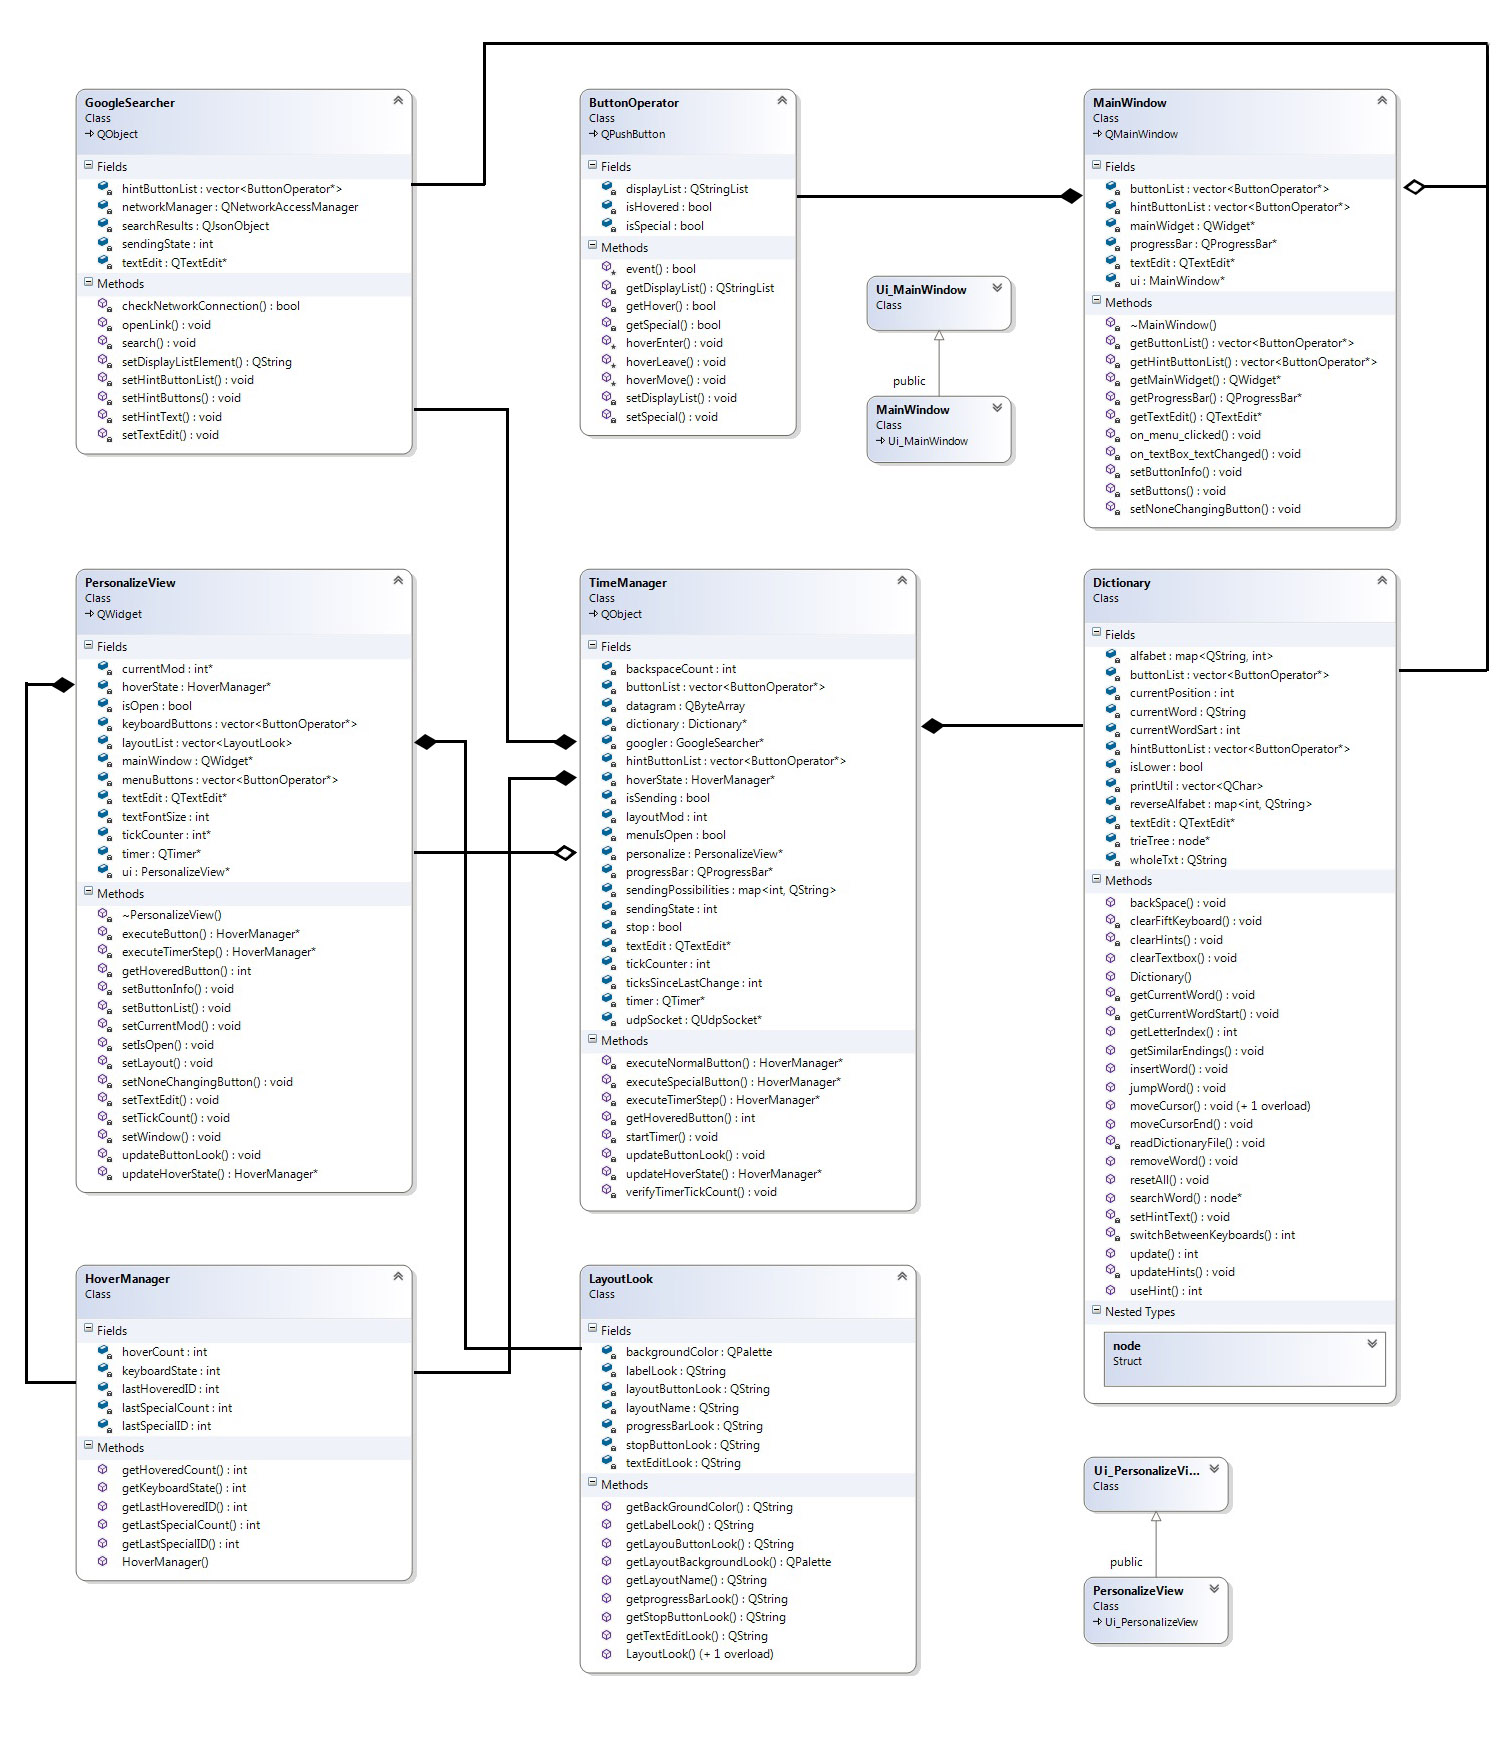
\includegraphics[width=0.7\textwidth]{img/classDiagram.jpg}}
		\caption{Poglądowy diagram klas zaimplementowanych w projekcie.}
		\label{fig:classDiag}
		
\end{figure}
\section{Opis klas zastosowanych}\label{sec:klas}

\section{Zaimplementowane algorytmy}\label{sec:algorytmy}
W poniższych podrozdziałach zaprezentowano zasadę działania zaimple\-men\-towanych w oprogramowaniu algorytmów. 
\subsection{Działanie przycisków}
W aplikacji każdy przycisk jest obiektem klasy ButtonOperator, która dzie\-dzi\-czy po klasie QPushButton. Dzięki czemu obiekty przycisków mogą ko\-rzy\-stać zarówno z metod klasy nadrzędnej np. isCheckable(), jak i klasy dzie\-dzi\-czącej. Właśnie dzięki nadpisaniu metod domyślnych klasy QPushButton  -  ho\-ver\-Enter() i hoverLeave() stworzono możliwość detekcji, nad którym przyciskiem aktualnie znajduje się punkt fiksacji wzroku. Podczas wywołania obu metod zmieniana jest wartość logiczna zmiennej isHovered aktualnie obserwowanego przycisku.  Prócz informacji o tym, czy dany przycisk jest aktualnie używany przechowuje się również dane o tym, czy przycisk zalicza się do tzw. ''spe\-cja\-lnych'', czy też nie, jak i listę dostępnych dla niego tekstów do wy\-świe\-tla\-nia – wyglądów przycisku dla 6 stanów kla\-wia\-tu\-ry (małe litery, duże litery, znaki specjalne karta pierwsza, znaki specjalne karta druga, polskie litery, menu kontekstowe). Wszystkie te dane wprowadza się podczas  uruchamiania kla\-wia\-tu\-ry i wtedy także przypisuje się przyciski kolejno do specjalnej listy. Kolejność jest znacząca w przypadku przycisków ''specjalnych'', gdyż ich obsługa zależna jest od wartości ich ID zapisanego w pliku ze stałymi. 
Określenie przycisku działającego odbywa się poprzez sprawdzenie jego ID, którego zmienna isHovered jest prawdziwa w klasie TimeManager. Do zarządzania stanem kla\-wia\-tu\-ry, o\-sta\-tnio wybranym przyciskiem specjalnym oraz ostatnio obserwowanym przyciskiem powstała klasa HoverManager. Zbiera ona na bieżąco informację o  ID przycisku ostatnio najechanego, o tym przez jaki czas dany przycisk jest już pod punktem fiksacji, o aktualnym stanie kla\-wia\-tu\-ry, o os\-ta\-tnio wybranym spe\-cja\-lnym przycisku (np. CapsLock) oraz przez jaki czas działanie tego przycisku się utrzymuje. Większość z tych danych odświeżana jest co 200ms (stała zde\-fi\-nio\-wa\-na w pliku ze stałymi) podczas każdego wykonywania się metody TimerStep(). Jej działanie przedstawiono za pomocą pseudokodu ~\ref{sec:alg1}.
\begin{algorithm}
\caption{Działanie funkcji TimerStep()}
\label{sec:alg1}
\begin{algorithmic}
\STATE pobierz ID aktualnie fiksowanego przycisku
\IF{pobrane ID różne jest od -1}
\IF{zwykłe przyciski są w trybie wstrzymania}
\IF{jeśli aktualnie fiksowany przycisk jest specjalny}
\STATE hoverState (obiekt klasy HoverManager) ustaw aktualnie aktywny przycisk na pobrane ID
\STATE Wykonaj krok timera (funkcja executeTimerStep())
\STATE Pokaż czas przez jaki przycisk jest fiksowany na pasku postępu dla informacji użytkownika.
\ENDIF
\ELSE
\STATE Wykonaj powyższe funkcje dla wszystkich przycisków - niezależnie od tego, czy są specjalne, czy nie.
\ENDIF
\ENDIF
\STATE Wywołaj funkcję verifyTimerTickCount().
\end{algorithmic}
\end{algorithm}
\\Zadaniem wyżej wspomnianej funkcji \-executeTimerStep() jest sprawdzenie, czy dany przycisk był fiksowany przez odpowiednią ilość czas (zmienna, której wartość zależy od ilości pomyłek popełnionych przez użytkownika, jest dynamicznie zmieniana podczas korzystania z klawiatury – analizowane to jest w funkcji ve\-ri\-fyTimerTickCount()). Jeżeli warunek ten został spełniony to dalszy przebieg działań zależy od tego, czy przycisk był specjalny, czy też nie oraz czy klawiatura nie znajduje się w trybie wstrzymania. 
\subsubsection{Działanie przycisków specjalnych}
W tabeli ~\ref{table:specialButtons} wymieniono wszystkie specjalne przyciski z widoku klawiatury oraz opisano po krótce algorytm ich działania. W tabeli ~\ref{table:specialButtonsMenu} przedstawiono przyciski widoku menu oraz ich zachowanie.

\begin{table}
    \begin{tabular}{|p{4cm}|p{8.5cm}|}
        \hline
    \textbf{Nazwa przycisku} & \textbf{Działanie}\\ \hline
     Backspace & Wywołuję metodą backspace() klasy Dictionary, której działanie opisano w podrozdziale ~\ref{sec:backspc}.\\ \hline
    CapsLock & W przypadku pierwszego wciśnięcia zmienia stan kla\-wia\-tu\-ry z 0 na 1 i utrzymuje ją dopóki nie zostanie wybrany po raz wtóry lub wykonana zostanie czynność innego przycisku zmieniającego stan klawiatury. \\ \hline
 Czyść & Korzysta z metody resetAll() klasy \-Dictionary i po\-wo\-du\-je czyszczenie edytora tekstowego oraz z nim związanych zmiennych jak currentPosition, currentWord, currentWordSart, wholeTxt (więcej na ten temat w rozdziale ~\ref{sec:text}).\\ \hline
Menu & Otwiera okno klasy Personalize.\\ \hline
Przesuń się o jedno słów w prawo lub w lewo & Wywołuje funkcje jumpWord() klasy Dictionary, która powoduje przesunięcie się kursora na koniec po\-prze\-dnie\-go słowa, lub na początek kolejnego. Każdorazowo zmieniana jest wartość zmie\-nnej currentWord i wholeText.~\ref{sec:text}\\ \hline
 Przesuń się w kierunku początku tekstu (home) lub na jego koniec (end) & Wybranie przycisku powoduje przesunięcie się kursora w jednym z dwóch kierunków oraz zmiane wartości zmie\-nnej wholeText i currentWord (~\ref{sec:text}). \\ \hline
 Przyciski podpowiedzi & Wyświetlane są na nich podpowiedzi, których tworzenie opisane jest w rodziale ~\ref{sec:trietree}. Ich użycie powoduje zastąpienie aktualnie wpisywanej frazy auto uzupełnionym słowem pobranym ze słownika. \\ \hline
  Shift & W przypadku wciśnięcia zmieniony zostaje stan kla\-wia\-tu\-ry z 0 na 1, a po użyciu przycisku ze znakiem stan kla\-wia\-tu\-ry wraca do stanu 0. \\ \hline
   Stop i start & Wprowadza kla\-wia\-tu\-rę w stan wstrzymania lub w stan pracy. W zależności od wartości zmiennej isStop jest możliwe, lub nie, korzystanie z przycisków ze znakami.\\ \hline
   Strzałka w lewo i prawo &  Korzystając z metody moveCursor klasy Dictionary przemieszcza kursor o jeden znak w danym kierunku. Może zmienić wartość currentWord (~\ref{sec:text}) korzystając z metod getCurrentWord() oraz getCurrentWordStart()(~\ref{sec:alg2}) opisanych w późniejszych rozdziałach.\\ \hline
     Wyjdź & Powoduje opuszczenie aplikacji.\\ \hline 
      Wyszukaj na podanej platformie & Przyciśniecie przycisku powoduje sprawdzenie połączenia internetowego, a następnie wysłanie wpisanej treści pola tekstowego do funkcji search() klasy GoogleSearcher. ~\ref{sec:searcher}\\ \hline
        Wyślij & Wysyła dotychczas wpisany tekst na broadcast na port 45454 za pomocą metody writeDatagram() klasy QUdpSocket.\\ \hline
    Zmiana trybu wyszukiwania & Strzałki powodują na zmianę trybu wyszukiwania. Do wyboru ''Google'', ''YouTube'', ''Filmweb''. Zmieniają wartość zmiennej sendingState niezbędnej do popranego działania funkcji  search() klasy GoogleSearcher.~\ref{sec:searcher}\\ \hline 
    Znaki specjalne & Zmienia stan kla\-wia\-tury na odpowiednio 2 i 3 przy ko\-lej\-nych kliknięciach. \\ \hline
       \end{tabular}
    \caption{Lista specjalnych przycisków wraz z ich działaniem.} 
    \label{table:specialButtons}
\end{table}
\begin{table}
    \begin{tabular}{|p{4cm}|p{8.5cm}|}
        \hline
    \textbf{Nazwa przycisku} & \textbf{Działanie}\\ \hline
       Strzałki zmieniające aktualną wartość progową czasu fiksacji & Strzałki powodują zmniejszenie lub zwiększenie wartości zmiennej tickCounter przechowującej ilość 200ms interwałów, po upływie których (w przypadku braku zmiany fiksowanego punktu) przycisk można uznać za wciśnięty. Początkowo czas ten wynosi 3s, jednak w wyniku dynamicznej korekty następuje zmniejszenie lub zwiększenie liczby tych interwałów. Korekta uruchamia się, gdy użytkownik przekroczy dopuszczalną ilość błędów w ciągu minuty. Więcej na temat dynamicznej zmiany czasu w podrozdziale ~\ref{sec:dynamic}. \\ \hline  
       Strzałki zmieniające wielkość czcionki w edytorze tekstu & Strzałki powodują zamianę właściwości edytora tekstu. \\ \hline
       Strzałki zmieniające wygląd aplikacji & Użytkownik może wybrać między jednym z 5 wersji kolorystycznych poprzez dynamiczną zmianę wyglądu na podstawie danych z listy i aktualnego indeksu.  \\ \hline    
       Wyjście & Powoduje zamknięcie okna menu. \\ \hline
    \end{tabular}
    \caption{Lista specjalnych przycisków z menu w raz z ich działaniem.} 
    \label{table:specialButtonsMenu}
\end{table}



Jako wciśnięcie rozumie się tu czas fiksacji nad przyciskiem przekracający progową wartość. Stany klawiatury to odpowiednio 0-małe litery, 1-wielkie litery, 2-znaki specjalne strona pierwsza, 3-zanki specjalne strona druga,\\4-polskie znaki, 5-menu kontekstowe dla polskich znaków.
\subsubsection{Działanie przycisków nomalnych}
Za wpisywanie znaków z klawiatury do edytora odpowiedzialna jest funkcja \-update() klasy Dictionary. Jest ona głównym zarządcą jeśli chodzi o wprowadzanie znaków w odpowiedniej pozycji. W pierwszej kolejności sprawdzane jest, czy stan klawiatury różny jest od stanu piątego (menu kontekstowe). Gdy spełniony jest dany warunek to porównywana jest aktualnie wprowadzana wartość z u\-prze\-dnio wprowadzoną. Wyjątek stanowi pierwsze wprowadzenie znaku do e\-dy\-to\-ra. W przypadku dwóch identycznych liter czyszczona jest zawartość piątego stanu klawiatury i przechodzi się do wywołania funkcji switchBetweenKeyboards(), która zwraca informację o tym, czy stan kla\-wia\-tu\-ry się zmienił. Tam sprawdzane jest, czy wprowadzony znak jest jedną z liter posiadających polskie odpo\-wie\-dni\-ki tj. \textit{a-ą, c-ć, e-ę, l-ł, n-ń, o-ó, s-ś, z-ż-ź}. Gdy znajdzie się on wśród wymienionej listy, to dla odpowiadającego przycisku ustawiany jest test dla klawiatury stanu piątego i następuje jej wyświetlenie. Działanie takiego zachowania widać na rysunkach 
 ~\ref{fig:startA},~\ref{fig:doubleA}.
\begin{figure}[!h]
		\centering
		\scalebox{.7}{
		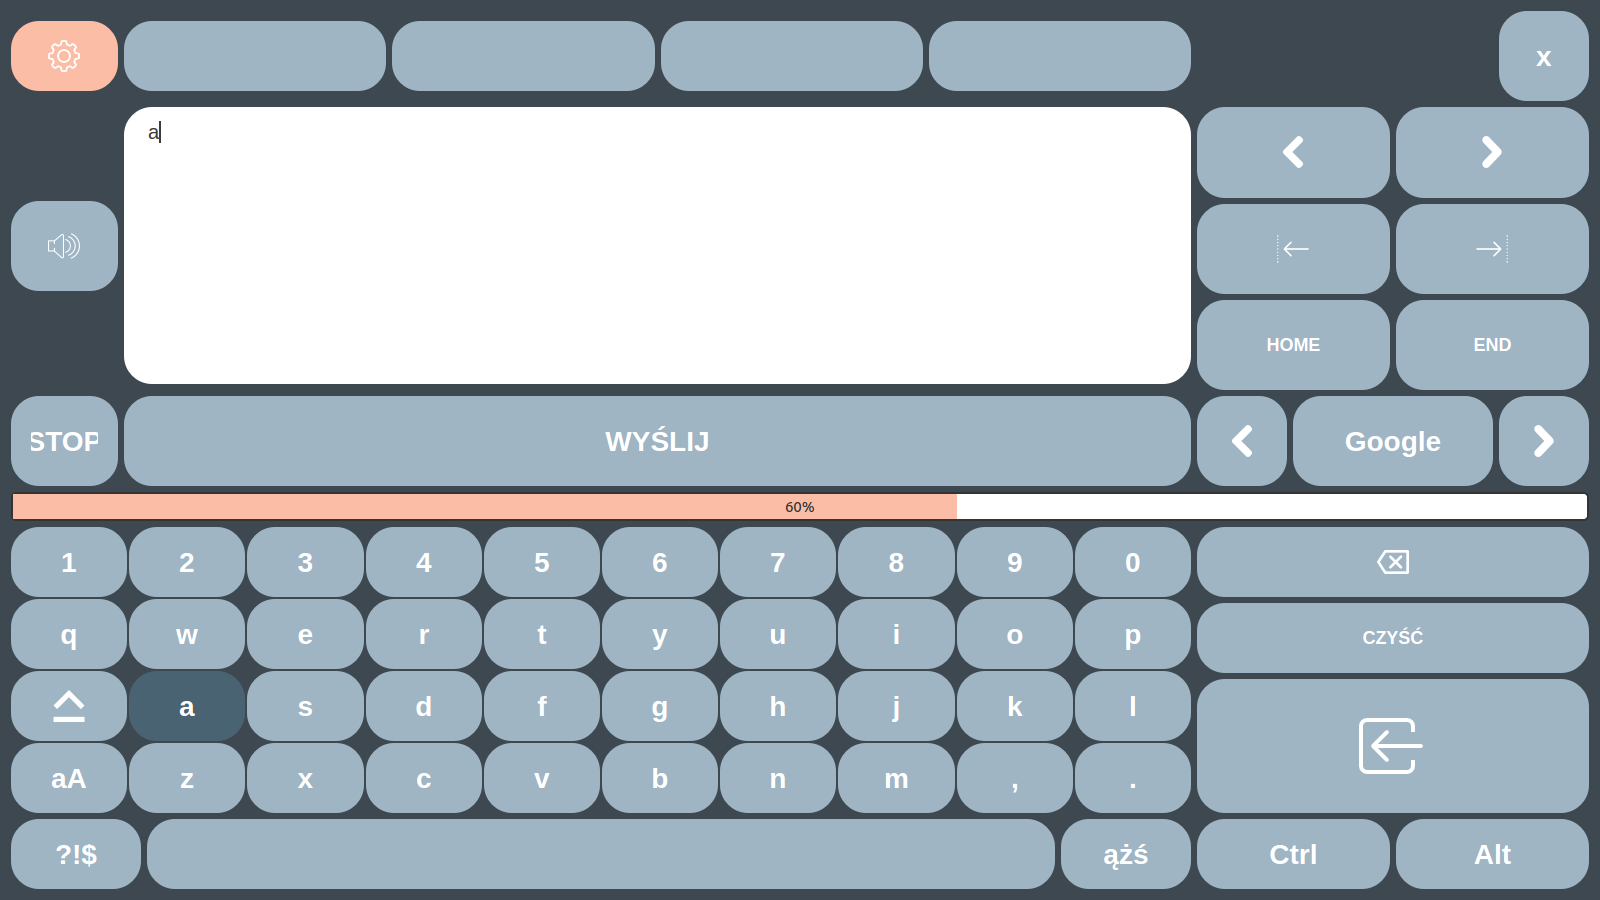
\includegraphics[width=1\textwidth]{img/startA.jpg}}
		\caption{Widok aplikacji z klawiatura w stanie zerowym po wpisaniu litery 'a'.}
		\label{fig:startA}
\end{figure}
\begin{figure}[!h]
		\centering
		\scalebox{.7}{
		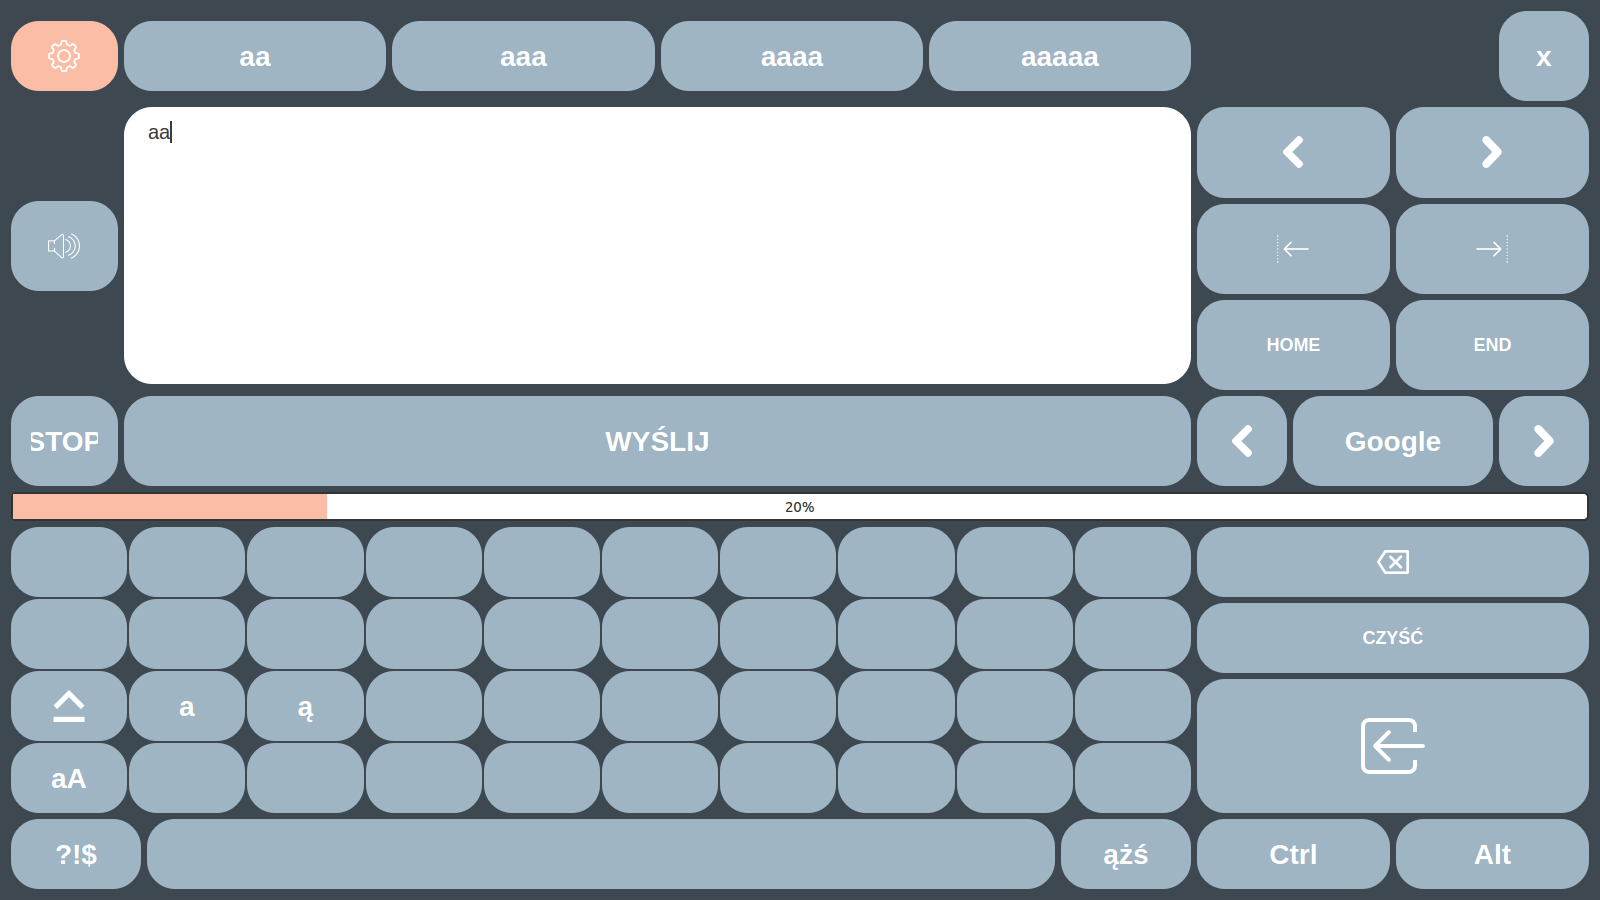
\includegraphics[width=1\textwidth]{img/doubleA.jpg}}
		\caption{Widok aplikacji z klawiaturą w stanie piątym po wpisaniu drugiej litery 'a'.}
		\label{fig:doubleA}
\end{figure}\\
W innym wypadku aktualna litera dopisywana jest do aktualnie tworzonoego słowa (currentWord), kursor przesuwany jest o jedną pozycję w prawo. Gdy dodana jest spacja aktualnie przetwarzane słowo jest uznawane za skończone i zapamiętywany jest nowy początek kolejnego słowa. Odświeżony zostaje również widok podpowiedzi, których powstawanie omówiono w późniejszym rozdziale ~\ref{sec:trietree}.
W sytuacji, gdy wybrana zostaje litera z menu kontekstowego (klawiatury w stanie piątym), to albo wpisany tekst zostaje podmieniony na polską literę,lub nie ulega zmianie. Przykładowo po wpisaniu ''aa'' użytkownik po raz kolejny wybiera literę ''a'' - tzn. planował wpisanie frazy ''aa''. Jeśli jednak decyduje się na literę ''ą'', to w miejsce widniejącego napisu ''aa'' pojawia się ''ą''.
Poglądowy diagram przepływu przedstawiono no rysunku ~\ref{fig:wordFlow}.
\begin{figure}[!h]
		\centering
		\scalebox{1}{
		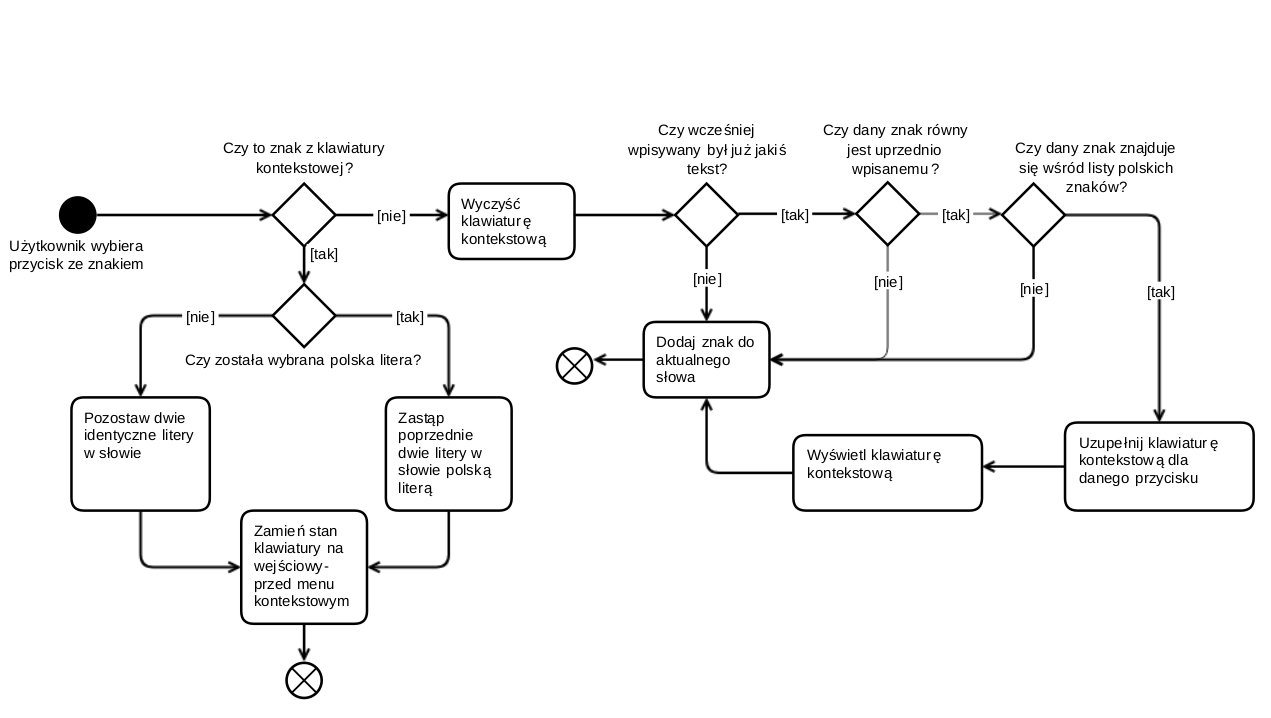
\includegraphics[width=1\textwidth]{img/writeFlow.jpg}}
		\caption{Widok aplikacji z klawiaturą w stanie piątym po wpisaniu drugiej litery 'a'.}
		\label{fig:wordFlow}
\end{figure}
\subsection{Praca z tekstem}~\label{sec:text}
Wpisywanie tekstu w aplikacji odbywa się poprzez specjalny algorytm kontrolujący zawartość aktualnie pisanego słowa oraz całego tekstu. W czasie działania programu, w pamięci przechowywany jest currentWord, czyli aktualne słowo tj. ciąg znaków, liter lub cyfr, które zaczynają się na początku wpisywanego tekstu lub po spacji, a kończą się w pozycji kursora. Dodanie spacji po ciągu znaków kończy słowo i usuwa je ze zmiennej currentWord, a dodaje do zmiennej zwanej wholeText, która przechowuje dotychczas wpisany tekst. Przykładowo jeśli mamy tekst jak na rysunku ~\ref{fig:sentence} to w zmiennej wholeText przechowywujemy ''''Wymagajcie od siebie choćby inni od was nie wymagali.'' ~Jan Paweł II '', a w currentWord ''sie''. W ten sposób podpowiedzi generowane będą jedynie dla cząstki ''sie'', a tekst wpisywany będzie w pozycji kursora, która również monitorowana jest przez zmienną currentPosition. Scalenie wholeText i currenWord następuję, gdy zmieniamy pozycję kursora strzałkami, lub jeśli do tekstu dodana zostanie spacja, a za kursorem nie znajduje się żaden znak. Przykład przedstawia rysunek ~\ref{fig:sentence2}. 
\begin{figure}[!h]
		\centering
		\scalebox{1}{
		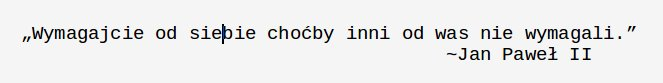
\includegraphics[width=1\textwidth]{img/sentence.jpg}}
		\caption{Przykładowe zapisywanie tekstu do zmiennych w zależności od pozycji kursora.}
		\label{fig:sentence}
\end{figure}
\begin{figure}[!h]
		\centering
		\scalebox{1}{
		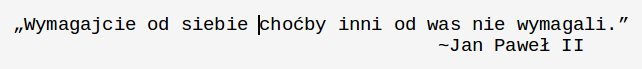
\includegraphics[width=1\textwidth]{img/sentence2.jpg}}
		\caption{Przykładowe zapisywanie tekstu do zmiennych w zależności od pozycji kursora.}
		\label{fig:sentence2}
\end{figure}

Zmienna currentWord została zespolona z wholeText poprzez wklenie jej na pozycji zapisanej jako currentWordStart. 
W celu dynamicznego ustalania pozycji currentWordStart oraz zawartości currentWord powstały funkcje: getCurrentWordStart() oraz getCurrentWord(). Działanie pierwszej zademonstrowano za pomocą pseudokodu ~\ref{sec:alg2}.
\begin{algorithm}
\caption{Działanie funkcji getCurrentWordStart()}
\label{sec:alg2}
\begin{algorithmic}
\IF{currentWord nie jest pusty \&\&  currentPosition nie jest  na początku tekstu}
\FOR{każda pozycja aż do początku tekstu}
\STATE pobierz literę z wholeText w danej pozycji
\IF{pobrana wartość nie jest liczbą ani literą}
\STATE $currentWordStart = dana pozycja + 1$
\ENDIF
\ENDFOR
\ENDIF
\end{algorithmic}
\end{algorithm}\\
Działanie drugiej sprowadza się do wycięcia faragmentu tekstu między currentWordStart, zaimplementowanym w wyniku działania poprzedniej funkcji, a currentPosition.
\subsubsection{Usuwanie znaków} \label{sec:backspc}
Proces usuwania znaków staje się trudniejszy ze względu na ułatwiające kontrolę nad tekstem currentWord i wholeText. Pier\-wszym napotkanym problemem była sytuacja, w której currentWord jest puste. W takim wypadku należy usunąć znak znajdujący się w currentPosition ze zmie\-nnej wholeText, a następnie za pomocą wcześniej opisanych funkcji getCurrentWordStart() oraz getCurrentWord() otrzymać informację o nowej wartości currentWord. Kolejnym krokiem jest wycięcie wartości zmiennej currentWord z wholeText, przesunięcie kursora dla informacji użytkownika w odpowiednią pozycję oraz odświeżenie wyglądu podpowiedzi.
Gdy currentWord ma wartość, sytuacja upraszcza się do usunięcia ostatniego znaku z currentWord. W celu reprezentacji tekstu dla użytkownika należy scalić wholeText z currentWord, ale by nie utracić wartości wholeText stworzono tymczasową zmienną currentText, który zawiera całą treść wpisanego tekstu.
\subsection{Trie tree}\label{sec:trietree}
Jak wyżej ~\ref{sec:trie}  wspomniano, w pracy wykorzystano drzewo typu Trie w celu pracy z rozległym słownikiem. Słowa z pliku w formacie TXT wczytywane są do programu podczas uruchamiania klawiatury- każda z linii dostarczanego pliku powinna stanowić pojedynczy wyraz. Słowa te, za pomocą sztucznie wy\-ge\-ne\-ro\-wa\-nych list kodujących oraz dekodujących polski alfabet, wprowadzane są do drzewa typu Trie. Drzewo takie powstaje poprzez stworzenie pustego węzła typu node - struktury zadeklarowanej w pliku nagłówkowym klasy obsługującej współpracę ze słownikiem – Dictionary. Struktura node przechowuje informacje o rodzicu bieżącego węzła, o jego potomkach – czyli węzłach następujących oraz wektor zawierający informację o przynależności danego węzła literowego do słowa. 
Po zainicjowaniu węzła zerowego, po kolei analizowane są słowa ze sło\-wni\-ka w funkcji insertWord().Każde jest rozpatrywane jako tablica liter (char) \\i iteracyjnie następuje najpierw kodowanie litery na odpowiadający jej indeks (za pomocą  mapy alfabet), potem, sprawdzane jest, czy w drzewie nie istnieje już węzeł odpowiadający danej wartości. Gdy nie znaleziono gałęzi drzewa pasujących do poszukiwanej wartości tworzy się za pomocą funkcji calloc przestrzeń w pamięci na przyszłe dzieci tego węzła, a jako ich rodzica podaje się aktualnie przeglądany węzeł z literą. Kolejno, niezależnie od wyniku uprzednio rozpatrywanego warunku, o ile słowo wciąż posiada litery do przeglądu, przenosi się \\o poziom niżej w drzewie ( na poziom dziecka  uprzednio rozpatrywanej litery) \\i proces zachodzi od początku.  Gdy przetworzono wszystkie litery słowa do listy wystąpień ostatniego odwiedzonego węzła dopisany zostaje indeks słowa \\w słowniku – tym samym oznaczając jego koniec. Na rysunku ~\ref{fig:insertWord} przed\-sta\-wio\-no, w sposób graficzny, działanie danej funkcji.
\begin{figure}[!h]
		\centering
		\scalebox{1}{
		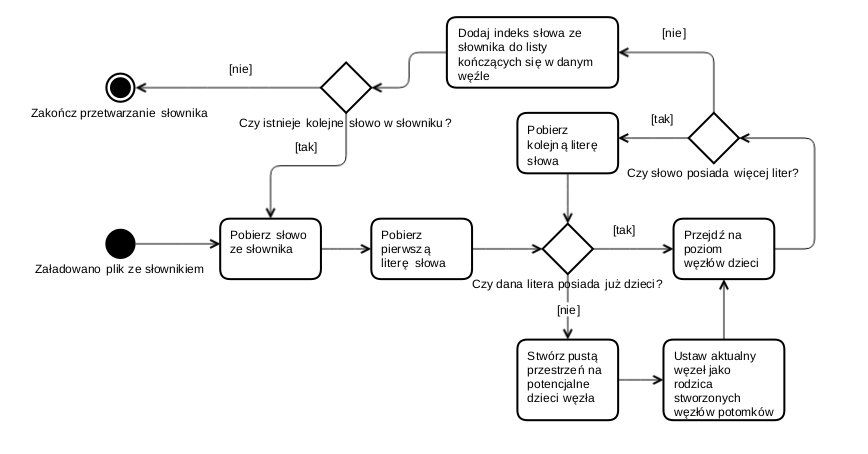
\includegraphics[width=1\textwidth]{img/insertWordFlow.jpg}}
		\caption{Diagram przepływu dla funkcji insertWord() wprowadzającej słowa do drzewa typu Trie. }
		\label{fig:insertWord}
\end{figure}

Po uzupełnieniu słownika nastąpić może auto uzupełnianie wpisywanego tekstu.
Każde wpisanie litery powoduje wywołanie metody updateHints(), która jest odpowiedzialna za tworzenie oraz wyświetlanie podpowiedzi, zgodnie \\z wprowadzonym do tej pory słowem. Jako poszukiwaną frazę traktujemy ciąg znaków, które użytkownik wpisał do pozycji kursora od ostatniej spacji, bądź początku tekstu. W wypadku, gdy ten ciąg znaków jest dłuższy niż dwa, wykorzystywana jest funkcja komunikująca się ze stworzonym słownikiem – searchWord(). Przekazywane jest drzewo Trie słownika oraz aktualnie poszukiwana fraza (bez formatowania). 
Wpisywana fraza, również traktowana jest jako zbiór liter, które przeglądane są jedna po drugiej. Dla każdej następuje zmiana dzięki mapie kodującej alfabet na odpowiadający indeks, który umożliwia przeszukiwanie słownika. Sprawdzane jest, czy istnieje potomek drzewa Trie o danym indeksie – jeśli tak, to następuje zmiana węzła na węzeł dziecka, tak, że przy przeszukiwaniu drzewa będą brane pod uwagę jedynie węzły z rodzicem będącym pierwszą literą poszukiwanej frazy. Gdy przeszuka się wszystkie litery, bądź w trakcie tego procesu zabraknie węzłów potomków dla danej kombinacji liter to zwracany jest odpowiednio ostatni węzeł wspólny dla danej frazy lub też węzeł pusty. 

W celu lepszego zrozumienia działania algorytmu rozpatrzmy go na przykładzie. Załóżmy, że mamy drzewo takie jak na rysunku ~\ref{fig:trie}. Jeśli wyszukamy frazę ''ko'' to funkcja zwróci nam węzeł i jego dzieci. Możliwe auto uzupełnienia wyglądają wtedy tak jak na rysunku ~\ref{fig:trieKO}.
\begin{figure}[!h]
		\centering
		\scalebox{.5}{
		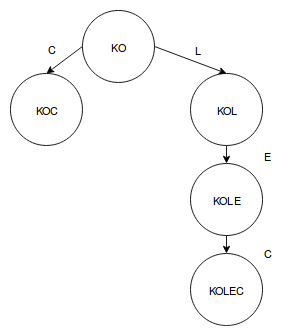
\includegraphics[width=1\textwidth]{img/trieKO.jpg}}
		\caption{Przykładowy węzeł do autouzupełniania słów po wpisaniu frazy ''ko''. }
		\label{fig:trieKO}
		\end{figure}
Złożenie końcówek wyrazów zachodzi w funkcji getSimilarEndings(), której przekazywany jest znaleziony
 węzeł, pusty wektor, do którego mają zostać zapisane wynikowe wyrazy oraz węzeł znaków niezbędny do dekodowania. 
W pierwszym kroku sprawdzane jest, czy w danym węźle kończą się  jakieś słowa, jeśli tak (wektor wystąpień węzła jest różny od zera), \\to każdą literę zapisaną w wyżej wymienionym wektorze znaków zapisuje się do jednego słowa (tworząc końcówkę do auto uzupełniania). Gotowy ciąg znaków zapisywany jest do wektora z końcówkami. W wypadku pierwszego wykonania się funkcji mamy do czynienia z pustym wektorem znaków- toteż nie zostanie stwo\-rzo\-na żadna końcówka. Nawet jeśli  ‘’ko’’ było pełną formą słowa nie powinna się ona wyświetlać w proponowanych opcjach użytkownika. Aby uzupełnić we\-ktor znaków należy przejrzeć przesłany węzeł (ten z rysunku ~\ref{fig:trieKO}) – w tym celu sprawdza się, czy dzieci węzła odpowiadającej każdej literze alfabetu nie są puste, gdyż programowe drzewo ma, prócz wcześniej przedstawionych gałęzi, jeszcze 33 (zakładając, że zaimplementowany alfabet posiada 35 liter) nieobdarzone wartością gałęzie przedstawione na rysunku ~\ref{fig:trieKOnull}. Gdy znaleziono element o niezerowej wartości pobierana jest za pomocą mapy symetrycznej (reverseAlfabet) wartość literowa węzła i wprowadzana jest do wektora znaków. Węzeł z ‘’ko’’ zmieniany jest w węzeł pierwszego pierwszego dziecka – w tym wypadku ‘’koc’’. Następnie przez rekurencję ponownie rozpoczyna się sprawdzanie, czy dane słowo kończy się w tym węźle. Jeśli tak, to proces zachodzi według powyżej opisanych kroków, jeśli nie, to znów poszukiwany jest węzeł potomny z kolejną literą końcówki słowa do auto uzupełniania. Algorytm przedstawiono w sposób graficzny na rysunku ~\ref{fig:similarEndingsFlow}
		\begin{figure}[!h]
		\centering
		\scalebox{.9}{
		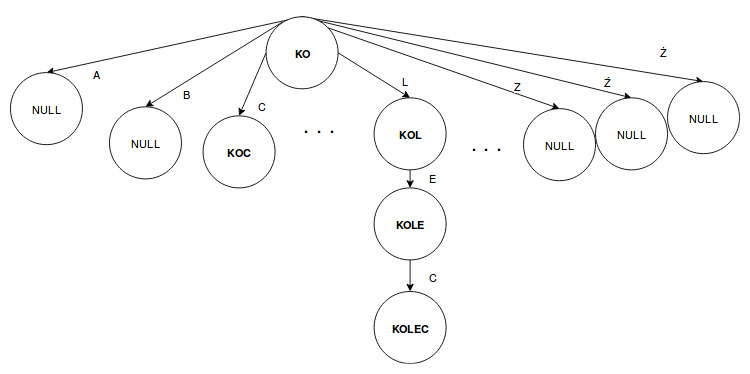
\includegraphics[width=1\textwidth]{img/trieKOnull.jpg}}
		\caption{Reprezentacja przykładowego węzła widzianego w programie. }
		\label{fig:trieKOnull}
		\end{figure}
				\begin{figure}[!h]
		\centering
		\scalebox{1}{
		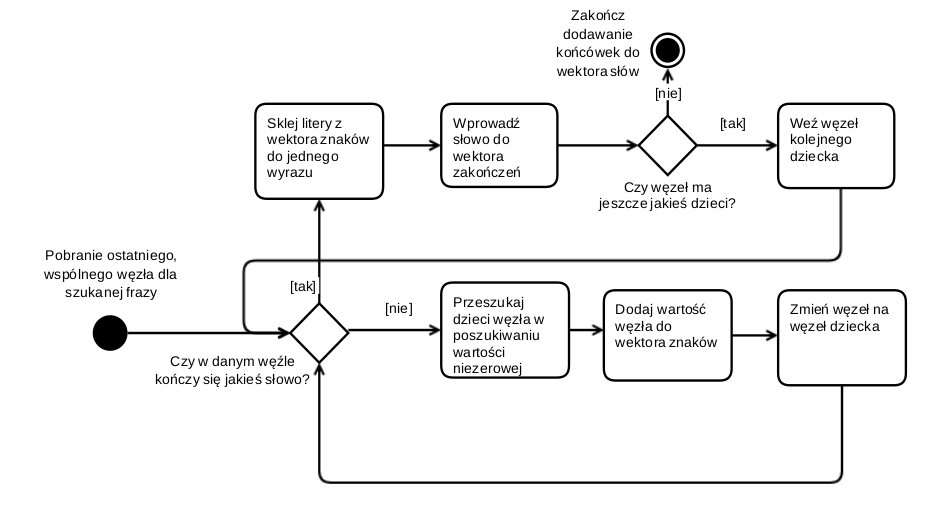
\includegraphics[width=1\textwidth]{img/similarEndingsFlow.jpg}}
		\caption{Diagram przepływu dla funkcji getSmiliarEndings().}
		\label{fig:similarEndingsFlow}
		\end{figure}\\
Ostatnim krokiem w stworzeniu podpowiedzi jest skrócenie listy końcówek do liczby przycisków przeznaczonych na podpowiedzi oraz zespolenie ich z dotychczas wpisanym słowem. Taki ciąg znaków można przedstawić użytkownikowi jako napis na przycisku, który po wybraniu wpisuje reprezentowany tekst do pola tekstowego zamieniając dotychczasową frazę na wybraną oraz dodając znak spacji na końcu nowowybranego słowa.
\subsection{Dynamiczna zmiana czasu progowego fiksacji}\label{sec:dynamic}
Jak wspomniano wcześniej klawiatura umożliwia dynamiczną zmianę czasu czasu progowego fiksacji (decydującego o tym kiedy dany przycisk zostanie wywołany). Zmiana następuję w oparciu o ilość błędów wykonanych przez użytkownika w określonym oknie czasowym. Weryfikacja następuję co minutę. Jeśli w tym czasie użytkownik popełni 5 lub więcej błedów (użyje przycisku Backspace), to czas fiksacji ulegnie wydłużeniu o jedną sekundę. Pięć błedów stanowi, dla ustawień początkowych, czyli progowego czasu fiksacji ustawionego na 3s, 25\% znaków wpisanych w tym czasie. Dla ilości błędów mniejszej niż dwa czas fiksacji zostaje skrócony. Jeśli użtkownik użyje przycisku Backspace 3-4 razy w ciągu minut czas progowy fiksacji nie ulegnie zmianie. Czas fiksacji został ograniczony obu\-stro\-nnie poprzez stałe z pliku const.h. Założono, że nie może on być krótszy niż 1s i dłuższy niż 6s. Użytkownik ma również możliwość manualnego ustawienia czasu progowego, poprzez zmianę wartości w oknie menu.  

\subsection{Korzystanie z wyszukiwarki internetowej}\label{sec:searcher}
W celu pracy z przeglądarką niezbędne jest podłączenie drugiego ekranu, na którym może się otwierać okno przeglądarki. W innym wypadku okno kla\-wia\-tu\-ry ulegnie minimalizacji i nie ma możliwości powrotu do okna.

W przypadku skorzystania z jednego z trybów wysłania (''Google'', \\''YouTube'', ''Filmweb'') wywoływana jest metoda, GoogleSearcher, search(). W zależności od przesłanej wartości sendingState, informującego o tym, gdzie wysłane ma być zapytanie, do wyszukiwanego tekstu (pobranego z pola tekstowego) dołączana jest informacja, w którym serwisie szukać wyników. Taka informacja załączana jest jako argument uzupełniający URL powstały przez stworzenie spersonalizownej wyszukiwarki, dzięki spe\-cja\-lne\-mu Google API. Następnie obiekt klasy QNetworkAccessManager wywołuję metodę RESTową GET na obiekcie klasy QNetworkRequest, który za argument konstruktora przyjmuje powstałe URL z paramatrem.
\subsubsection{Google Api}
Jak już wcześniej wspomniano ~\ref{sec:customSearch} do projektu wykorzystano specjalne API Google - Google Custom Search Engine. Dzięki temu powstał specjalny link URL umożliwiający przyjmowanie różnych parametrów jako zapytanie do wyszukiwaraki. Co więcej specjalne API na rządanie GET zwraca iformację w postaci QNetworkReply, gdzie funkcja handleNetworkData() umożliwia jego przetworzenie w ustrukturyzowaną postać JSON. Obiekt JSON zawiera 10 pierwszych wynków wyszukiwania w specjalnej przeglądarce. Każdy z obiektów typu JSON posiada informacje o wyniku wyszukiwania. W skład takiego obiektu wchodzą ~\cite{googleJSON}:
\begin{itemize}
\item ''kind'': ''customsearch\#result''
\item ''title'': string
\item ''htmlTitle'': string
\item ''link'': string
\item ''displayLink'': string
\item ''snippet'': string
\item ''htmlSnippet'': string
\item  ''cacheId'': string
\item ''mime'': string,
\item ''fileFormat'': string
\item ''formattedUrl'': string
\item ''htmlFormattedUrl'': string
\item ''pagemap''
\end{itemize} 
Wykorzystując dane z ''title'' oraz ''link'' przedstawiane są użytkownikowi cztery pierwsze wyniki wyszukiwania w polu tekstowym,a ich wywołanie (otworzenie strony) odbywa się przez wybranie przystosowanych przycisków podpowiedzi \\z numerem wyniku wyszukiwania w przypadku wyszukiwania danych w Google. Przykład działania przedstawiono na rysunkach ~\ref{fig:googleSearch} oraz ~\ref{fig:searchResult}. 
			\begin{figure}[!h]
		\centering
		\scalebox{.7}{
		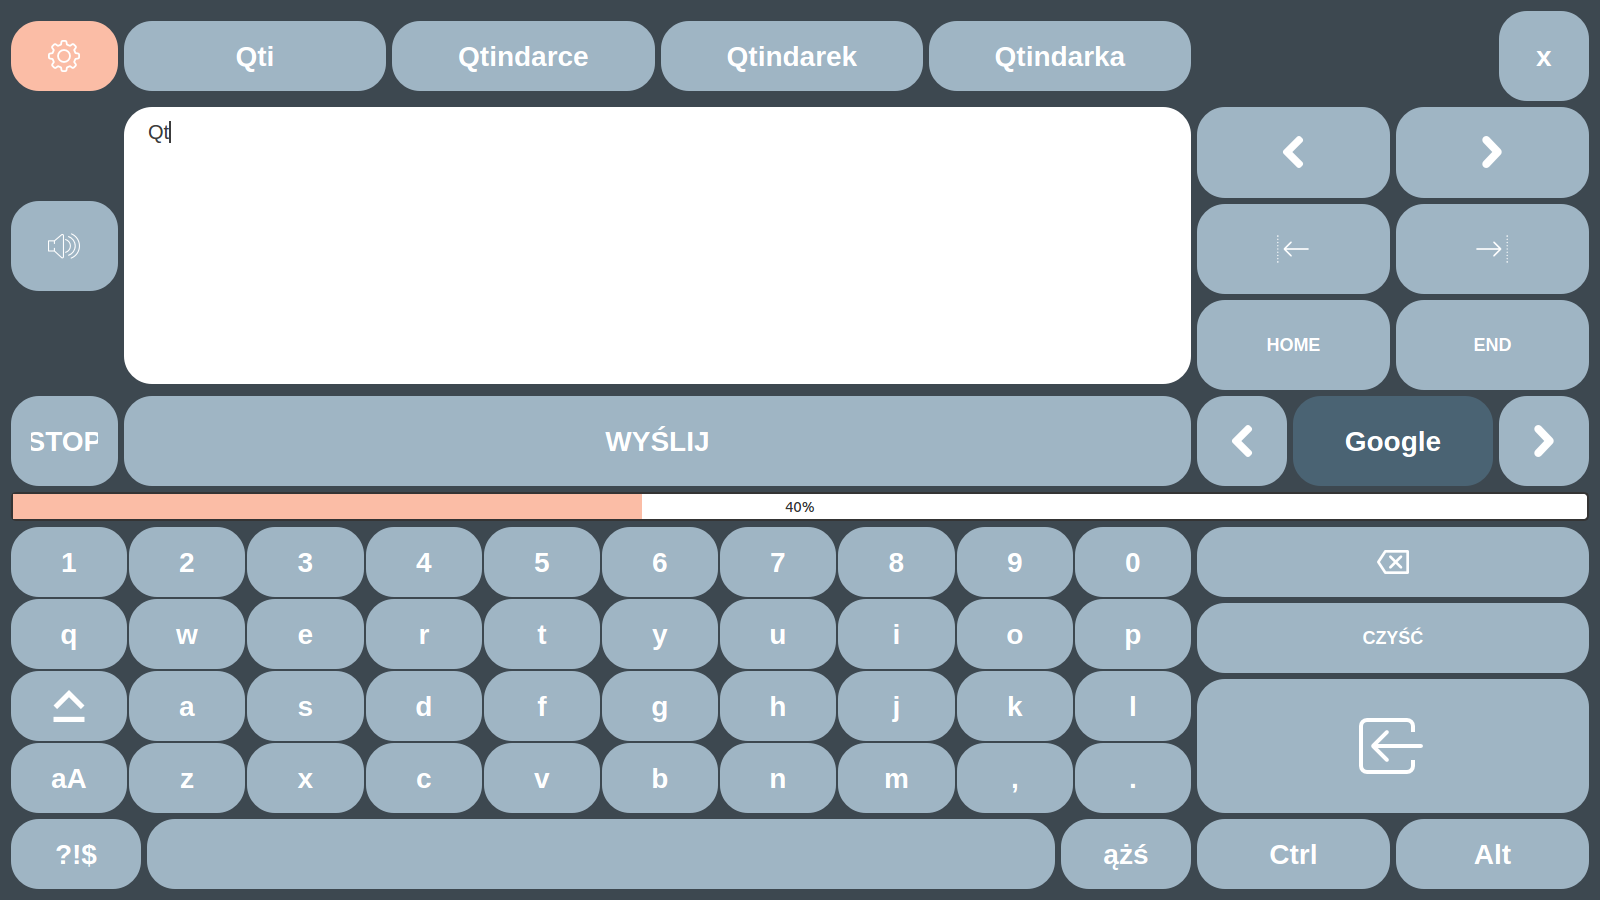
\includegraphics[width=1\textwidth]{img/qtSearch.jpg}}
		\caption{Przykładowy tekst wpisany do pola tekstowego, wysyłany jako argumnet wyszukiwania Google.}
		\label{fig:googleSearch}
		\end{figure}

	\begin{figure}
		\centering
		\scalebox{.7}{
		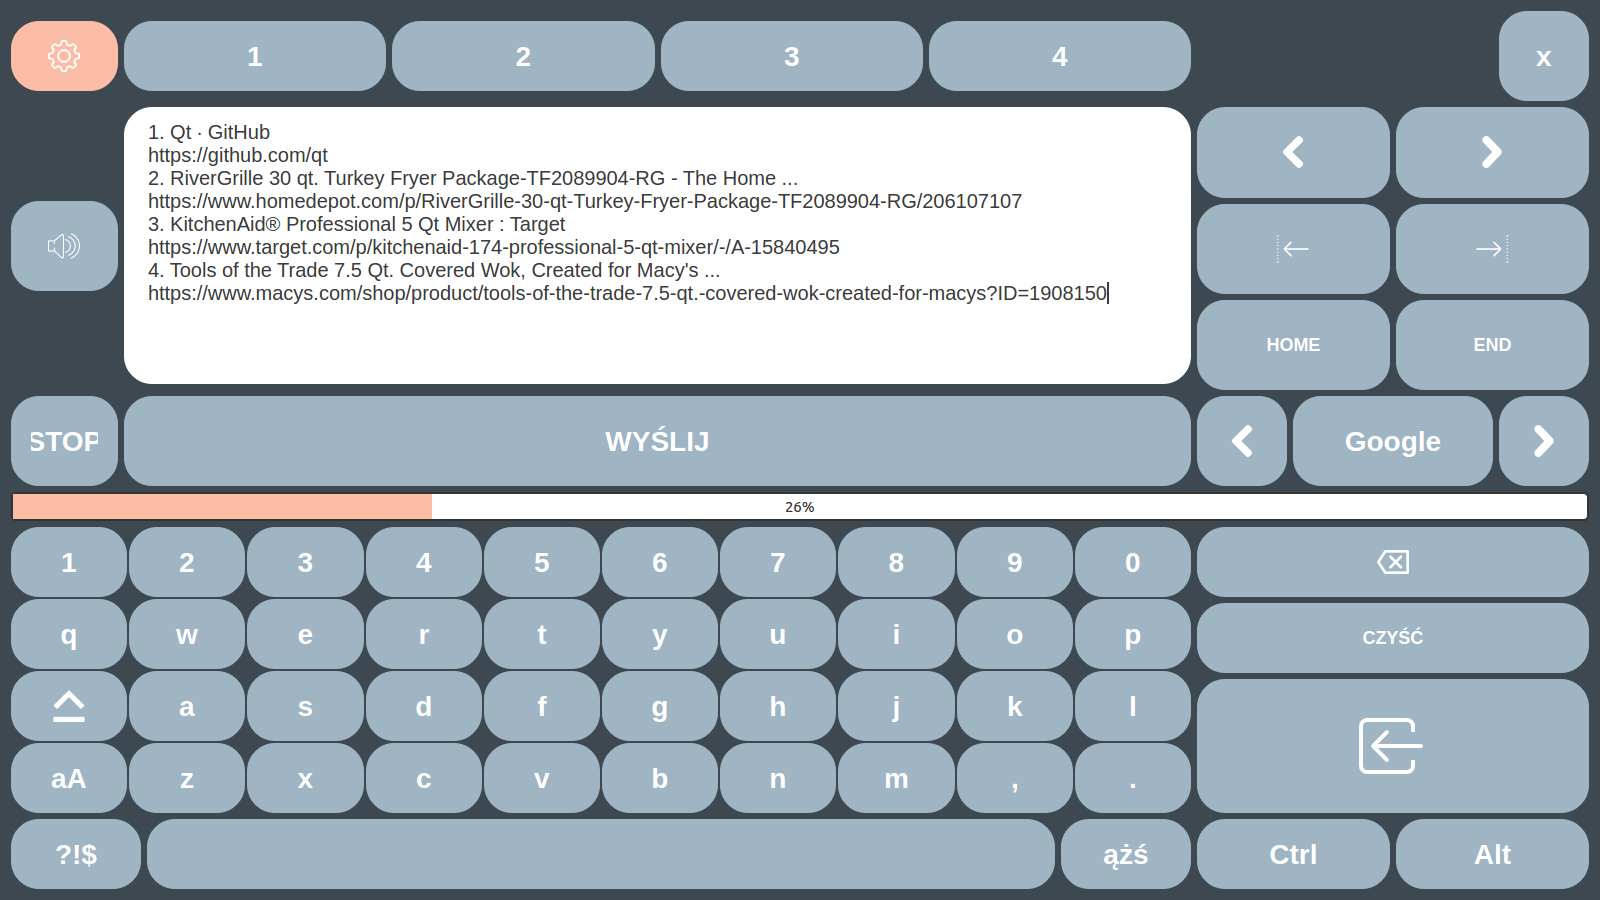
\includegraphics[width=1\textwidth]{img/qtsearchResult.jpg}}
		\caption{Wyniki wyszukiwana tekstu wpisanego na rysunku ~\ref{fig:googleSearch}.}
		\label{fig:searchResult}
		\end{figure}
W wypadku wyszukiwań w Youtube oraz Filmweb użytkownik nie ma możliwości wyboru  wyniku wyszukiwania - otwierany jest pierwszy wynik, który zawiera odpowiednie słowa kluczowe.

\section{Opis rozwiązania}
\section{Zaimplementowany interfejs użytkownika}
\end{document}


\chapter{Test i wyniki}
\chapter{Podsumowanie}




\bibliographystyle{unsrt}
\bibliography{bibliografia}


\end{document}